\documentclass[aspectratio=169,fleqn,xcolor={dvipsnames,table},handout]{beamer}
% Mit HU-Logo
%\usetheme[pageofpages=of,titlepagelogo=logo-huberlin-500]{hubln}
% Ohne HU-Logo
% Laut irgendwelcher internen Regularien darf das HU-Logo nicht von Studierenden benutzt werden
\usetheme[pageofpages=of]{hubln}

\usepackage[utf8]{inputenc}
\usepackage[T1]{fontenc}
\usepackage{tabularx}
\usepackage{hhline}
\usepackage{array}
\usepackage{tikz}
\usepackage{amsmath}
\usepackage{amssymb}
\usepackage{mathtools}
\usepackage{multirow}
\usepackage{minted}
%\usepackage{colortbl}
\usepackage{xcolor}
\usemintedstyle{monokai} %vs
%\definecolor{bg}{HTML}{282828}
\definecolor{bg}{RGB}{40, 40, 40}
\setminted{bgcolor=black,frame=lines,
               framesep=2mm}
\usefonttheme{professionalfonts}
\setbeamercovered{invisible}
\hfuzz=8.64pt % Antioverfullbox-inator

\setbeamercolor{block body alerted}{bg=alerted text.fg!10}
\setbeamercolor{block title alerted}{bg=alerted text.fg!20}
\setbeamercolor{block body}{bg=structure!10}
\setbeamercolor{block title}{bg=structure!20}
\setbeamercolor{block body example}{bg=green!10}
\setbeamercolor{block title example}{bg=green!20}
\setbeamertemplate{blocks}[rounded][shadow]

% Befehle für den Präsentationsmodus
% Die folgenden beiden Befehle erstellen eine Präsentation, die Notizen enthält und beim Öffnen auf zwei Bildschirmen auf einem die aktuelle Folie und auf dem anderen die nächste Folie und die Notizen anzeigt
% \setbeameroption{show notes}
% \setbeameroption{show notes on second screen=right}

% Anschließend diesen Befehl im Terminal nutzen
% w: in Fenstern statt Vollbild öffnen
% Switch-Screen, wenn Bildschirme zu vertauschen
% pdfpc --switch-screens --notes=right Presentation.pdf


% Einfügen von Notizen
% Hierfür muss nach einem Frame das folgende eingefügt werden
%\note[itemize]{
%    \item point 1
%    \item point 2
%}

% Dies ermöglicht es, eine stichpunktartige Notizenliste zu führen, die mit der vorhergehenden Folie zusammenhängt. Andere Notizsorten sind möglich, man möge hierfür die Dokumentation lesen

% \hypersetup{pdfpagemode=FullScreen}
% Dieser Befehl öffnet die Datei beim Öffnen direkt im Vollbildmodus


\newcommand{\newLine}{%
  \hfill\break
}

\tikzset{onslide/.code args={<#1>#2}{% from https://tex.stackexchange.com/a/6155/263192
  \only<#1>{\pgfkeysalso{#2}}
}}

\usetikzlibrary{positioning}

\pgfdeclarearrow{ %page 1020 of 3.0.1a manual
name = mmany,
parameters = { },
setup code = { },
drawing code = {
    \newdimen\arrowsize%
    \arrowsize=0.5pt%
    \pgfsetdash{}{+0pt}%
    \pgfsetmiterjoin%
    \advance\arrowsize by .25\pgflinewidth%
    \pgfpathmoveto{\pgfqpoint{0pt}{-9\arrowsize}}%
    \pgfpathlineto{\pgfqpoint{-13\arrowsize}{0pt}}%
    \pgfpathlineto{\pgfqpoint{0pt}{9\arrowsize}}%
    \pgfpathmoveto{\pgfqpoint{-19\arrowsize}{-10\arrowsize}}% 
    \pgfpathlineto{\pgfqpoint{-19\arrowsize}{10\arrowsize}}% 
    \pgfusepathqstroke%
    },
defaults = { }
}

\pgfdeclarearrow{ %page 1020 of 3.0.1a manual
name = omany,
parameters = { },
setup code = { },
drawing code = {
    \newdimen\arrowsize%
    \arrowsize=0.5pt%
    \pgfsetdash{}{+0pt}%
    \pgfsetmiterjoin%
    \advance\arrowsize by .25\pgflinewidth%
    \pgfpathmoveto{\pgfqpoint{0pt}{-9\arrowsize}}%
    \pgfpathlineto{\pgfqpoint{-13\arrowsize}{0pt}}%
    \pgfpathlineto{\pgfqpoint{0pt}{9\arrowsize}}%
    \pgfusepathqstroke%
    \pgfsetfillcolor{white}
    \pgfpathcircle{\pgfpoint{-19\arrowsize}{0}} {6\arrowsize}%
    \pgfusepathqfillstroke%
    },
defaults = { }
}

\pgfdeclarearrow{ %page 1020 of 3.0.1a manual
name = mone,
parameters = { },
setup code = { },
drawing code = {
    \newdimen\arrowsize%
    \arrowsize=0.5pt%%
    \pgfsetdash{}{+0pt}%
    \pgfsetmiterjoin%
    \advance\arrowsize by .25\pgflinewidth%
    \pgfpathmoveto{\pgfqpoint{-9\arrowsize}{-10\arrowsize}}% 
    \pgfpathlineto{\pgfqpoint{-9\arrowsize}{10\arrowsize}}% 
    \pgfpathmoveto{\pgfqpoint{-19\arrowsize}{-10\arrowsize}}% 
    \pgfpathlineto{\pgfqpoint{-19\arrowsize}{10\arrowsize}}%    
    \pgfusepathqstroke%
    },
defaults = { }
}

\pgfdeclarearrow{ %page 1020 of 3.0.1a manual
name = oone,
parameters = { },
setup code = { },
drawing code = {
    \newdimen\arrowsize%
    \arrowsize=0.5pt%
    \pgfsetdash{}{+0pt}%
    \pgfsetmiterjoin%
    \advance\arrowsize by .25\pgflinewidth
    \pgfpathmoveto{\pgfqpoint{-9\arrowsize}{-10\arrowsize}}% 
    \pgfpathlineto{\pgfqpoint{-9\arrowsize}{10\arrowsize}}% 
    \pgfsetfillcolor{white}
    \pgfpathcircle{\pgfpoint{-19\arrowsize}{0}} {6\arrowsize}%
    \pgfusepathqfillstroke%
    },
defaults = { }
}


% Hier die Daten zur Präsentation eintragen
\author[ls]{Lars Haukland (egentlig: Lukas Schramm)}
\title[sgp]{Kræsjkurs INF115}
\institute{Institutt for informatikk \\ Universitetet i Bergen}
\date[15.05.23]{15. Mai 2023}

% Dieses Dokument stellt nur die Präambel dar, alle Inhalte sind in die Datei Presentation.tex ausgelagert worden
\begin{document}
  % Diese Datei repräsentiert den Inhalt der Präsentation

% Titelseite
\begin{frame}[t,plain]
    \titlepage
\end{frame}

% table of contents
\section{Innføring}
\subsection*{Agenda}
\begin{frame}
    \tableofcontents
\end{frame}

\begin{frame}{Lars' eksamensrelevansspekulasjon}
%\rowcolors{2}{gray!25}{white}
    \begin{tabular}{l|l}
    Tema & Antatt relevans (by Lars (egentlig Lukas), ikke stol på det)\\\hline\pause
    SQL & Kjempeultramegaviktig\\\pause
    Relasjonsalgebra & Bare småoppgaver\\\pause
    ER-Diagrammer & Viktig\\\pause
    Normalisasjon & Veldig viktig\\\pause
    Indekser & Potensielt viktig\\\pause
    Transaksjoner & Viktig\\\pause
    Databaseadministrasjon & Aner ikke\\\pause
    Webapplikasjoner med php & Uviktig (også i det reelle livet)\\\pause
    NoSQL, XML, JSON & Ingen programmering, potensielt kunnskapsspørsmål\\\pause
    Andre småtemaer & Aner ikke\\\pause
    Guest lectures & Kanskje?
    \end{tabular}
\end{frame}

\subsection*{Download PDFen}
\begin{frame}{Last meg ned}
    \begin{figure}
        \centering
        
\includegraphics[height = 4.9cm]{images/downloadqr.png}
        \caption{https://tinyurl.com/inf115v23}
        \label{fig:qrcode}
    \end{figure}
\end{frame}

\section{SQL}
\subsection*{Teamer}
\begin{frame}{Temaer}
\begin{itemize}
    \item Select
    \item Aggregation
    \item Joins
    \item Update
    \item Insert
    \item Delete
    \item Create and Drop Tables
    \item Datatyper
    \item Constraints
    \item Alt mulig
    \item SQL injections
\end{itemize}
\end{frame}

\subsection*{Enkle Select statements}
\begin{frame}[fragile]{Select}
\begin{minted}{sql}
SELECT director, COUNT(*) as c -- Kolonner
FROM movie                     -- Tabeller
WHERE country = "Dabendorf"    -- Betingelser
GROUP BY director              -- Gruppering etter kolonner 
HAVING c > 3                   -- Betingelser etter grupper
ORDER BY c DESC                -- Sortering etter kolonner
LIMIT 3;                       -- Velg de første n output linjene
\end{minted}
\end{frame}

\subsection*{Aggregasjonsfunksjoner}
\begin{frame}[fragile]{Aggregation}
\begin{itemize}[<+->]
    \item Count: Teller antall elementer
    \item Sum: Summerer verdier
    \item Avg: Gjennomsnitt av verdier (tilsvarer count/sum)
    \item Min: Minimum
    \item Max: Maksimum
    \item Alle aggregasjonsfunksjoner ignorerer NULL verdier
\end{itemize}
\end{frame}

\subsection*{Joins}
\begin{frame}[fragile]{Join (2 varianter)}
\begin{minted}{sql}
SELECT *                -- Varianter 1
FROM film, screening    -- Velg alle tabeller og bruk WHERE
WHERE film.film_id = screening.film_id;
\end{minted}
\pause
\begin{minted}{sql}
SELECT *                -- Varianter 2
FROM film               -- Velg en tabell og bruk JOIN og ON
JOIN screening ON film.film_id = screening.film_id;
\end{minted}
\end{frame}

\begin{frame}{Types of Joins}
\begin{itemize}[<+->]
    \item INNER JOIN: Alle rader som finnes i begge tabeller
    \item LEFT (OUTER) JOIN: Alle rader som finnes i begge tabeller og alt fra venstre tabellen
    \item RIGHT (OUTER) JOIN: Alle rader som finnes i begge tabeller og alt fra høyre tabellen
    \item FULL (OUTER) JOIN: Alt fra begge tabeller
    \item \textit{Alt} mener tilsvarende JOIN columns
    \item Ikke-eksisterende verdier fylles med NULL verdier
    \item \dots SELF JOIN, CROSS JOIN, NATURAL JOIN, \dots
\end{itemize}
\end{frame}

\begin{frame}{Venn Diagram}
    \begin{figure}
        \centering
        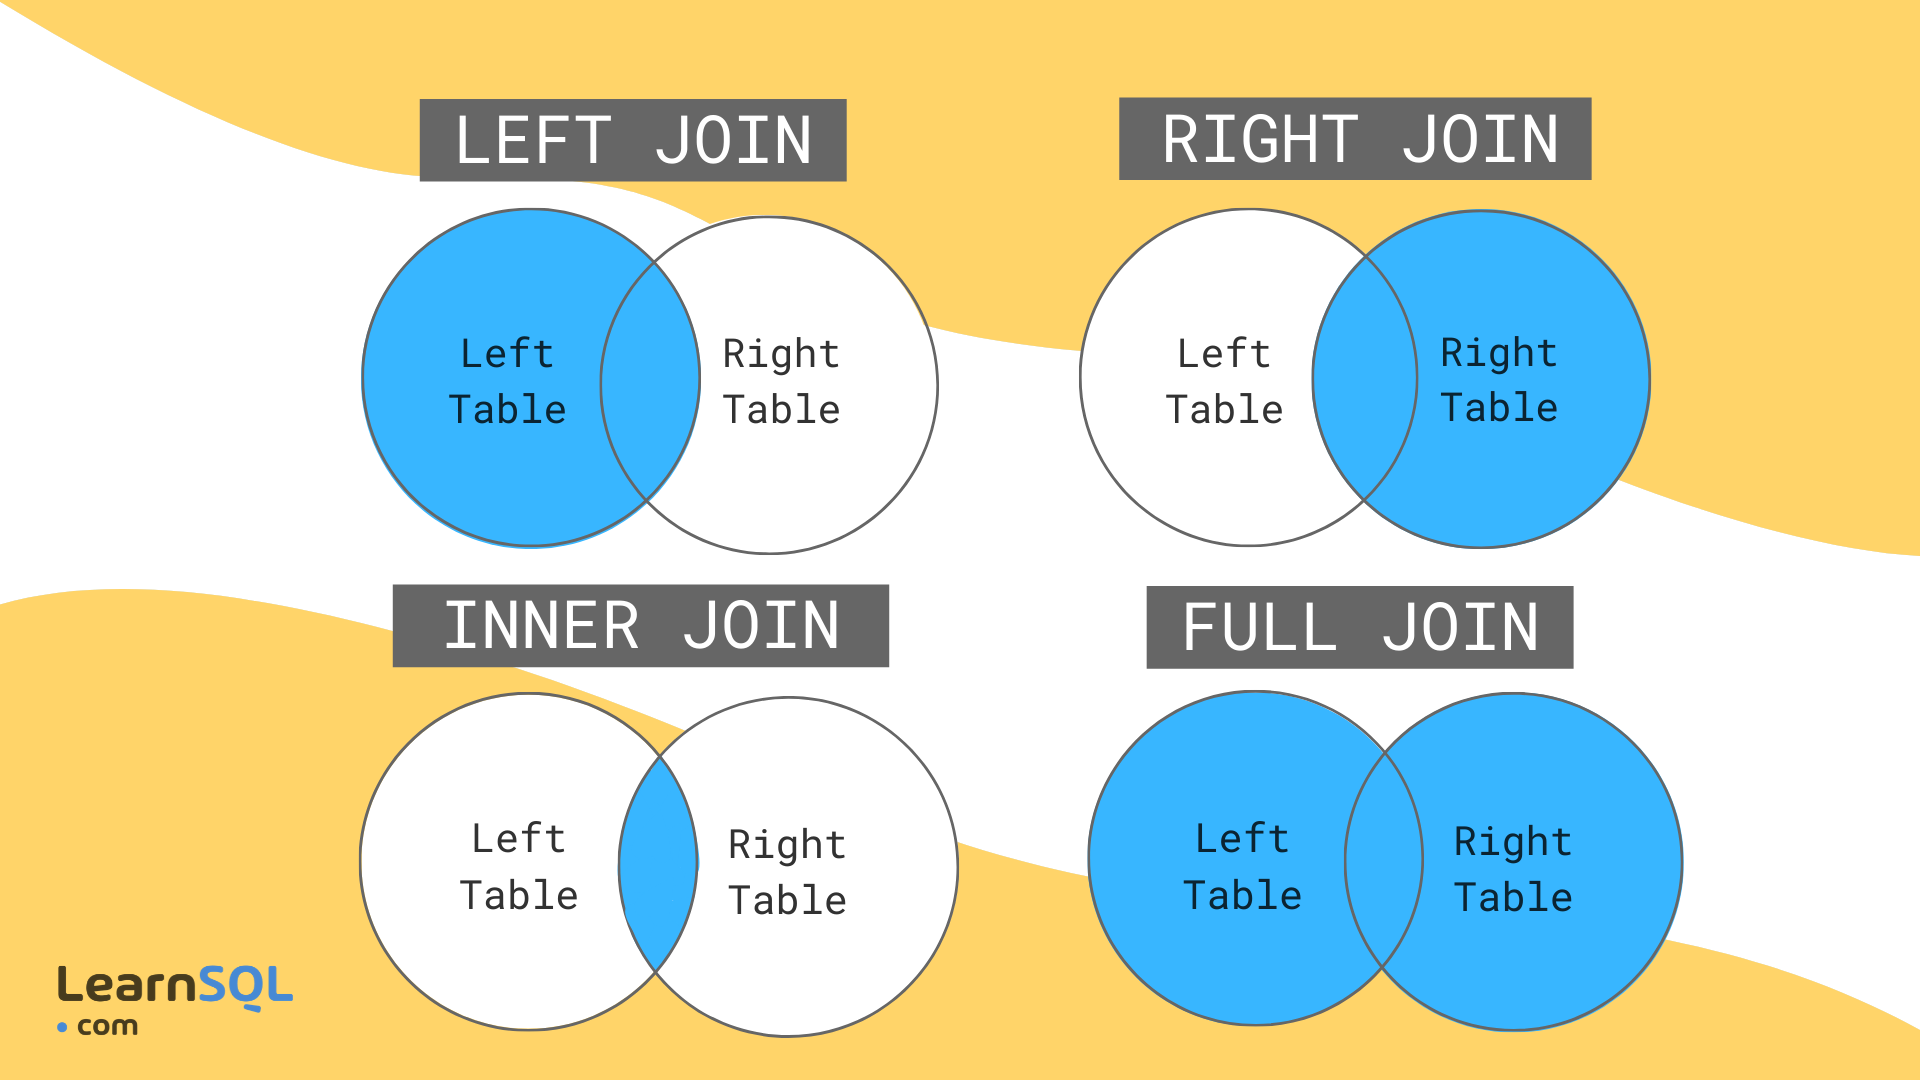
\includegraphics[height = 4.9cm]{images/joins.png}
        \caption{Kilde:
        https://learnsql.com/blog/learn-and-practice-sql-joins/}
        \label{fig:venndiagram}
    \end{figure}
\end{frame}

\begin{frame}%{Eksempel INNER JOIN}
\begin{columns}
    \begin{column}{0.48\textwidth}
        \begin{table}
        \resizebox{2.8cm}{!}{%
        \begin{tabular}{c|c|>{\columncolor[gray]{0.8}}c}
        RuteID & Fra & Til \\\hline
        0 & 2 & 1\\
        1 & 5 & 1\\
        2 & 1 & 2\\
        3 & 3 & 2\\
        4 & 2 & 3\\
        5 & 1 & 4\\
        6 & 1 & 6\\
        7 & 2 & 7
        \end{tabular}
        }
        \end{table}
		
		\vspace{0.2cm}
		
		\begin{table}
		\resizebox{3.5cm}{!}{%
		\begin{tabular}{>{\columncolor[gray]{0.8}}c|l}
		 FlyplassID & By\\\hline
		1 & Bergen\\
		2 & Dabendorf\\
		3 & PorsgruNN\\
		4 & Reykjavík\\
		5 & Oslo
		\end{tabular}
		}
		\end{table}
        
		
 	\end{column}
 	\pause
    \begin{column}{0.48\textwidth}
        \begin{table}
		\resizebox{6cm}{!}{%
		\begin{tabular}{c|c|>{\columncolor[gray]{0.8}}c|>{\columncolor[gray]{0.8}}c|l}
		 RuteID & Fra & Til & FlyplassID & By\\\hline
		 0 & 2 & 1 & 1 & Bergen\\
		 1 & 5 & 1 & 1 & Bergen\\
		 2 & 1 & 2 & 2 & Dabendorf\\
		 3 & 3 & 2 & 2 & Dabendorf\\
		 4 & 2 & 3 & 3 & PorsgruNN\\
		 5 & 1 & 4 & 4 & Reykjavík\\
		\end{tabular}
		}
		\caption{Eksempel: INNER JOIN}
		\end{table}
 	\end{column}
\end{columns}

\end{frame}

\begin{frame}%{Eksempel LEFT JOIN}
\begin{columns}
    \begin{column}{0.48\textwidth}
        \begin{table}
        \resizebox{2.8cm}{!}{%
        \begin{tabular}{c|c|>{\columncolor[gray]{0.8}}c}
        RuteID & Fra & Til \\\hline
        0 & 2 & 1\\
        1 & 5 & 1\\
        2 & 1 & 2\\
        3 & 3 & 2\\
        4 & 2 & 3\\
        5 & 1 & 4\\
        6 & 1 & 6\\
        7 & 2 & 7
        \end{tabular}
        }
        \end{table}
		
		\vspace{0.2cm}
		
		\begin{table}
		\resizebox{3.5cm}{!}{%
		\begin{tabular}{>{\columncolor[gray]{0.8}}c|l}
		 FlyplassID & By\\\hline
		1 & Bergen\\
		2 & Dabendorf\\
		3 & PorsgruNN\\
		4 & Reykjavík\\
		5 & Oslo
		\end{tabular}
		}
		\end{table}
        
		
 	\end{column}
 	\pause
    \begin{column}{0.48\textwidth}
        \begin{table}
		\resizebox{6cm}{!}{%
		\begin{tabular}{c|c|>{\columncolor[gray]{0.8}}c|>{\columncolor[gray]{0.8}}c|l}
		 RuteID & Fra & Til & FlyplassID & By\\\hline
		 0 & 2 & 1 & 1 & Bergen\\
		 1 & 5 & 1 & 1 & Bergen\\
		 2 & 1 & 2 & 2 & Dabendorf\\
		 3 & 3 & 2 & 2 & Dabendorf\\
		 4 & 2 & 3 & 3 & PorsgruNN\\
		 5 & 1 & 4 & 4 & Reykjavík\\
		 6 & 1 & 6 & NULL & NULL\\
         7 & 2 & 7 & NULL & NULL
		\end{tabular}
		}
		\caption{Eksempel: LEFT JOIN}
		\end{table}
 	\end{column}
\end{columns}
    
\end{frame}

\begin{frame}%{Eksempel RIGHT JOIN}
\begin{columns}
    \begin{column}{0.48\textwidth}
        \begin{table}
        \resizebox{2.8cm}{!}{%
        \begin{tabular}{c|c|>{\columncolor[gray]{0.8}}c}
        RuteID & Fra & Til \\\hline
        0 & 2 & 1\\
        1 & 5 & 1\\
        2 & 1 & 2\\
        3 & 3 & 2\\
        4 & 2 & 3\\
        5 & 1 & 4\\
        6 & 1 & 6\\
        7 & 2 & 7
        \end{tabular}
        }
        \end{table}
		
		\vspace{0.2cm}
		
		\begin{table}
		\resizebox{3.5cm}{!}{%
		\begin{tabular}{>{\columncolor[gray]{0.8}}c|l}
		 FlyplassID & By\\\hline
		1 & Bergen\\
		2 & Dabendorf\\
		3 & PorsgruNN\\
		4 & Reykjavík\\
		5 & Oslo
		\end{tabular}
		}
		\end{table}
        
		
 	\end{column}
 	\pause
    \begin{column}{0.48\textwidth}
        \begin{table}
		\resizebox{6cm}{!}{%
		\begin{tabular}{c|c|>{\columncolor[gray]{0.8}}c|>{\columncolor[gray]{0.8}}c|l}
		 RuteID & Fra & Til & FlyplassID & By\\\hline
		 0 & 2 & 1 & 1 & Bergen\\
		 1 & 5 & 1 & 1 & Bergen\\
		 2 & 1 & 2 & 2 & Dabendorf\\
		 3 & 3 & 2 & 2 & Dabendorf\\
		 4 & 2 & 3 & 3 & PorsgruNN\\
		 5 & 1 & 4 & 4 & Reykjavík\\
		 NULL & NULL & NULL & 5 & Oslo
		\end{tabular}
		}
		\caption{Eksempel: RIGHT JOIN}
		\end{table}
 	\end{column}
\end{columns}
    
\end{frame}

\begin{frame}%{Eksempel FULL OUTER JOIN}
\begin{columns}
    \begin{column}{0.48\textwidth}
        \begin{table}
        \resizebox{2.8cm}{!}{%
        \begin{tabular}{c|c|>{\columncolor[gray]{0.8}}c}
        RuteID & Fra & Til \\\hline
        0 & 2 & 1\\
        1 & 5 & 1\\
        2 & 1 & 2\\
        3 & 3 & 2\\
        4 & 2 & 3\\
        5 & 1 & 4\\
        6 & 1 & 6\\
        7 & 2 & 7
        \end{tabular}
        }
        \end{table}
		
		\vspace{0.2cm}
		
		\begin{table}
		\resizebox{3.5cm}{!}{%
		\begin{tabular}{>{\columncolor[gray]{0.8}}c|l}
		 FlyplassID & By\\\hline
		1 & Bergen\\
		2 & Dabendorf\\
		3 & PorsgruNN\\
		4 & Reykjavík\\
		5 & Oslo
		\end{tabular}
		}
		\end{table}
        
		
 	\end{column}
 	\pause
    \begin{column}{0.48\textwidth}
        \begin{table}
		\resizebox{6cm}{!}{%
		\begin{tabular}{c|c|>{\columncolor[gray]{0.8}}c|>{\columncolor[gray]{0.8}}c|l}
		 RuteID & Fra & Til & FlyplassID & By\\\hline
		 0 & 2 & 1 & 1 & Bergen\\
		 1 & 5 & 1 & 1 & Bergen\\
		 2 & 1 & 2 & 2 & Dabendorf\\
		 3 & 3 & 2 & 2 & Dabendorf\\
		 4 & 2 & 3 & 3 & PorsgruNN\\
		 5 & 1 & 4 & 4 & Reykjavík\\
		 6 & 1 & 6 & NULL & NULL\\
         7 & 2 & 7 & NULL & NULL\\
		 NULL & NULL & NULL & 5 & Oslo
		\end{tabular}
		}
		\caption{Eksempel: FULL OUTER JOIN}
		\end{table}
 	\end{column}
\end{columns}
    
\end{frame}


\subsection*{Oppdatere informasjoner}
\begin{frame}[fragile]{Update}
\begin{minted}{sql}
UPDATE book                 -- tabell
SET title = "Der satanarchäolügenialkohöllische Wunschpunsch"
WHERE book_id = 37;         -- betingelse
\end{minted}
\pause
\vspace{-5mm}
\begin{minted}{sql}
UPDATE music                -- tabell
SET title = "Supercalifragilisticexpialidocious",
   artist = "Mary Poppins"  -- oppdatert informasjon
WHERE song_id = 42;         -- betingelse
\end{minted}
\end{frame}

\subsection*{Legg til informasjoner}
\begin{frame}[fragile]{Insert (2 varianter)}
\begin{minted}{sql}
INSERT INTO film (film_id, title, director, genre)
VALUES (7, "Fantômas", "André Hunebelle", "Fransk tull"); 
\end{minted}
\pause
\begin{minted}{sql}
INSERT INTO film    -- kolonnenavn ikke nødvendig hvis alle blir brukt
VALUES (7, "Fantômas", "André Hunebelle", "Fransk tull"); 
\end{minted}
\end{frame}

\subsection*{Fjerne informasjoner}
\begin{frame}[fragile]{Delete}
\begin{minted}{sql}
DELETE FROM film        -- tabell
WHERE country = "USA";  -- betingelse
\end{minted}
\end{frame}

\subsection*{Lage nye tabeller}
\begin{frame}[fragile]{Create Table}
\begin{minted}{sql}
CREATE TABLE Persons (
Person_id int,              -- [column name] [datatype] [constraints]
    LastName varchar(40) NOT NULL,
    FirstName varchar(40),
    Age int,
    Department_id int UNIQUE,
    PRIMARY KEY (Person_id),    -- primær- og fremmednøkler
    FOREIGN KEY (Department_id) REFERENCES Department(Department_id),
    CHECK (Age>=18)             -- constraints
);
\end{minted}
\end{frame}

\subsection*{Slette tabeller}
\begin{frame}[fragile]{Drop Table}
\begin{minted}{sql}
DROP TABLE eksamenskarakterer;  -- tabell som skal slettes 
\end{minted}
\end{frame}

\subsection*{Datatyper}
\begin{frame}[fragile]{Datatyper}
\begin{minted}{sql}
char(20)            -- 20 tegn med fast lengde
varchar(20)         -- opptil 20 tegn
text                -- tekst med opptil 2^16 tegn
int                 -- integer (tinyint, smallint, bigint)
float(2)            -- float med 2 sifre bak komma
decimal(5,2)        -- 3 sifre før og 2 etter komma
enum ("INF102", "INF234", "INF237") -- en av n verdier
date                -- dato
timestamp           -- unix timestamp
\end{minted}
\end{frame}

\subsection*{Constraints}
\begin{frame}[fragile]{Constraints}
\begin{minted}{sql}
NOT NULL                    -- verdien er ikke NULL
UNIQUE                      -- kolonnen har ingen verdi flere ganger
PRIMARY KEY(key)            -- NOT NULL + UNIQUE
FOREIGN KEY(key) REFERENCES tabell(key) -- fremmednøkkel
AGE int CHECK (AGE >= 18)   -- betingelse
AGE int DEFAULT 18          -- standardverdi
\end{minted}
\end{frame}

\subsection*{Andre ting}
\begin{frame}[fragile]{Alt mulig}
\begin{minted}{sql}
SELECT DISTINCT                     -- fjerner duplikater
WHERE navn LIKE "A%"                -- alt som starter med A
-- % 0, 1 eller flere tegn
-- _ eksakt et tegn
WHERE category IN ("cake", "bread") -- verdien er i en liste
WHERE age BETWEEN 18 and 65         -- verdien er i en range
WHERE EXISTS (SELECT ...)           -- verdien finnes i en annen query
(SELECT ...) UNION (SELECT ...)     -- union av to queries
\end{minted}
\end{frame}

\begin{frame}[fragile]{Alt mulig}
\begin{minted}{sql}
SELECT Order_id, Price,
CASE    -- if betingelser i SELECT
    WHEN Price > 30 THEN "Won't pay freight"
    ELSE "Freight costs 10\$"
END AS FrightCost
FROM OrderDetails; 
\end{minted}
\end{frame}

\subsection*{SQL-Injections}
\begin{frame}{SQL-Injections}
    \begin{itemize}[<+->]
        \item Noen SQL kommandoer trenger input av brukeren
        \item Eksempel: Spørsmål etter brukernavn og passord
        \item Eksempel: Inputboks med søkebegrep i en søkefunksjon
        \item Hva skjer om brukeren taster inn onde ting?
        \item Programmerer må sjekke om input er farlig eller ikke
    \end{itemize}
\end{frame}

\begin{frame}[fragile]{}
\begin{minted}{python}
input_user = input()
commando1 = "SELECT * FROM Users WHERE name={input_user};"
execute_query(database, commando1)
\end{minted}
\pause
Input: lukas; DROP TABLE Users;
\pause
\begin{minted}{python}
commando1 = "SELECT * FROM Users WHERE name=lukas; DROP TABLE Users;"
execute_query(database, commando1)
\end{minted}
\pause
Brukeren har slettet brukertabellen. \pause Trist.
\end{frame}

\subsection*{Spørretid}
\begin{frame}{Spørsmål?}
    \begin{figure}
        \centering
        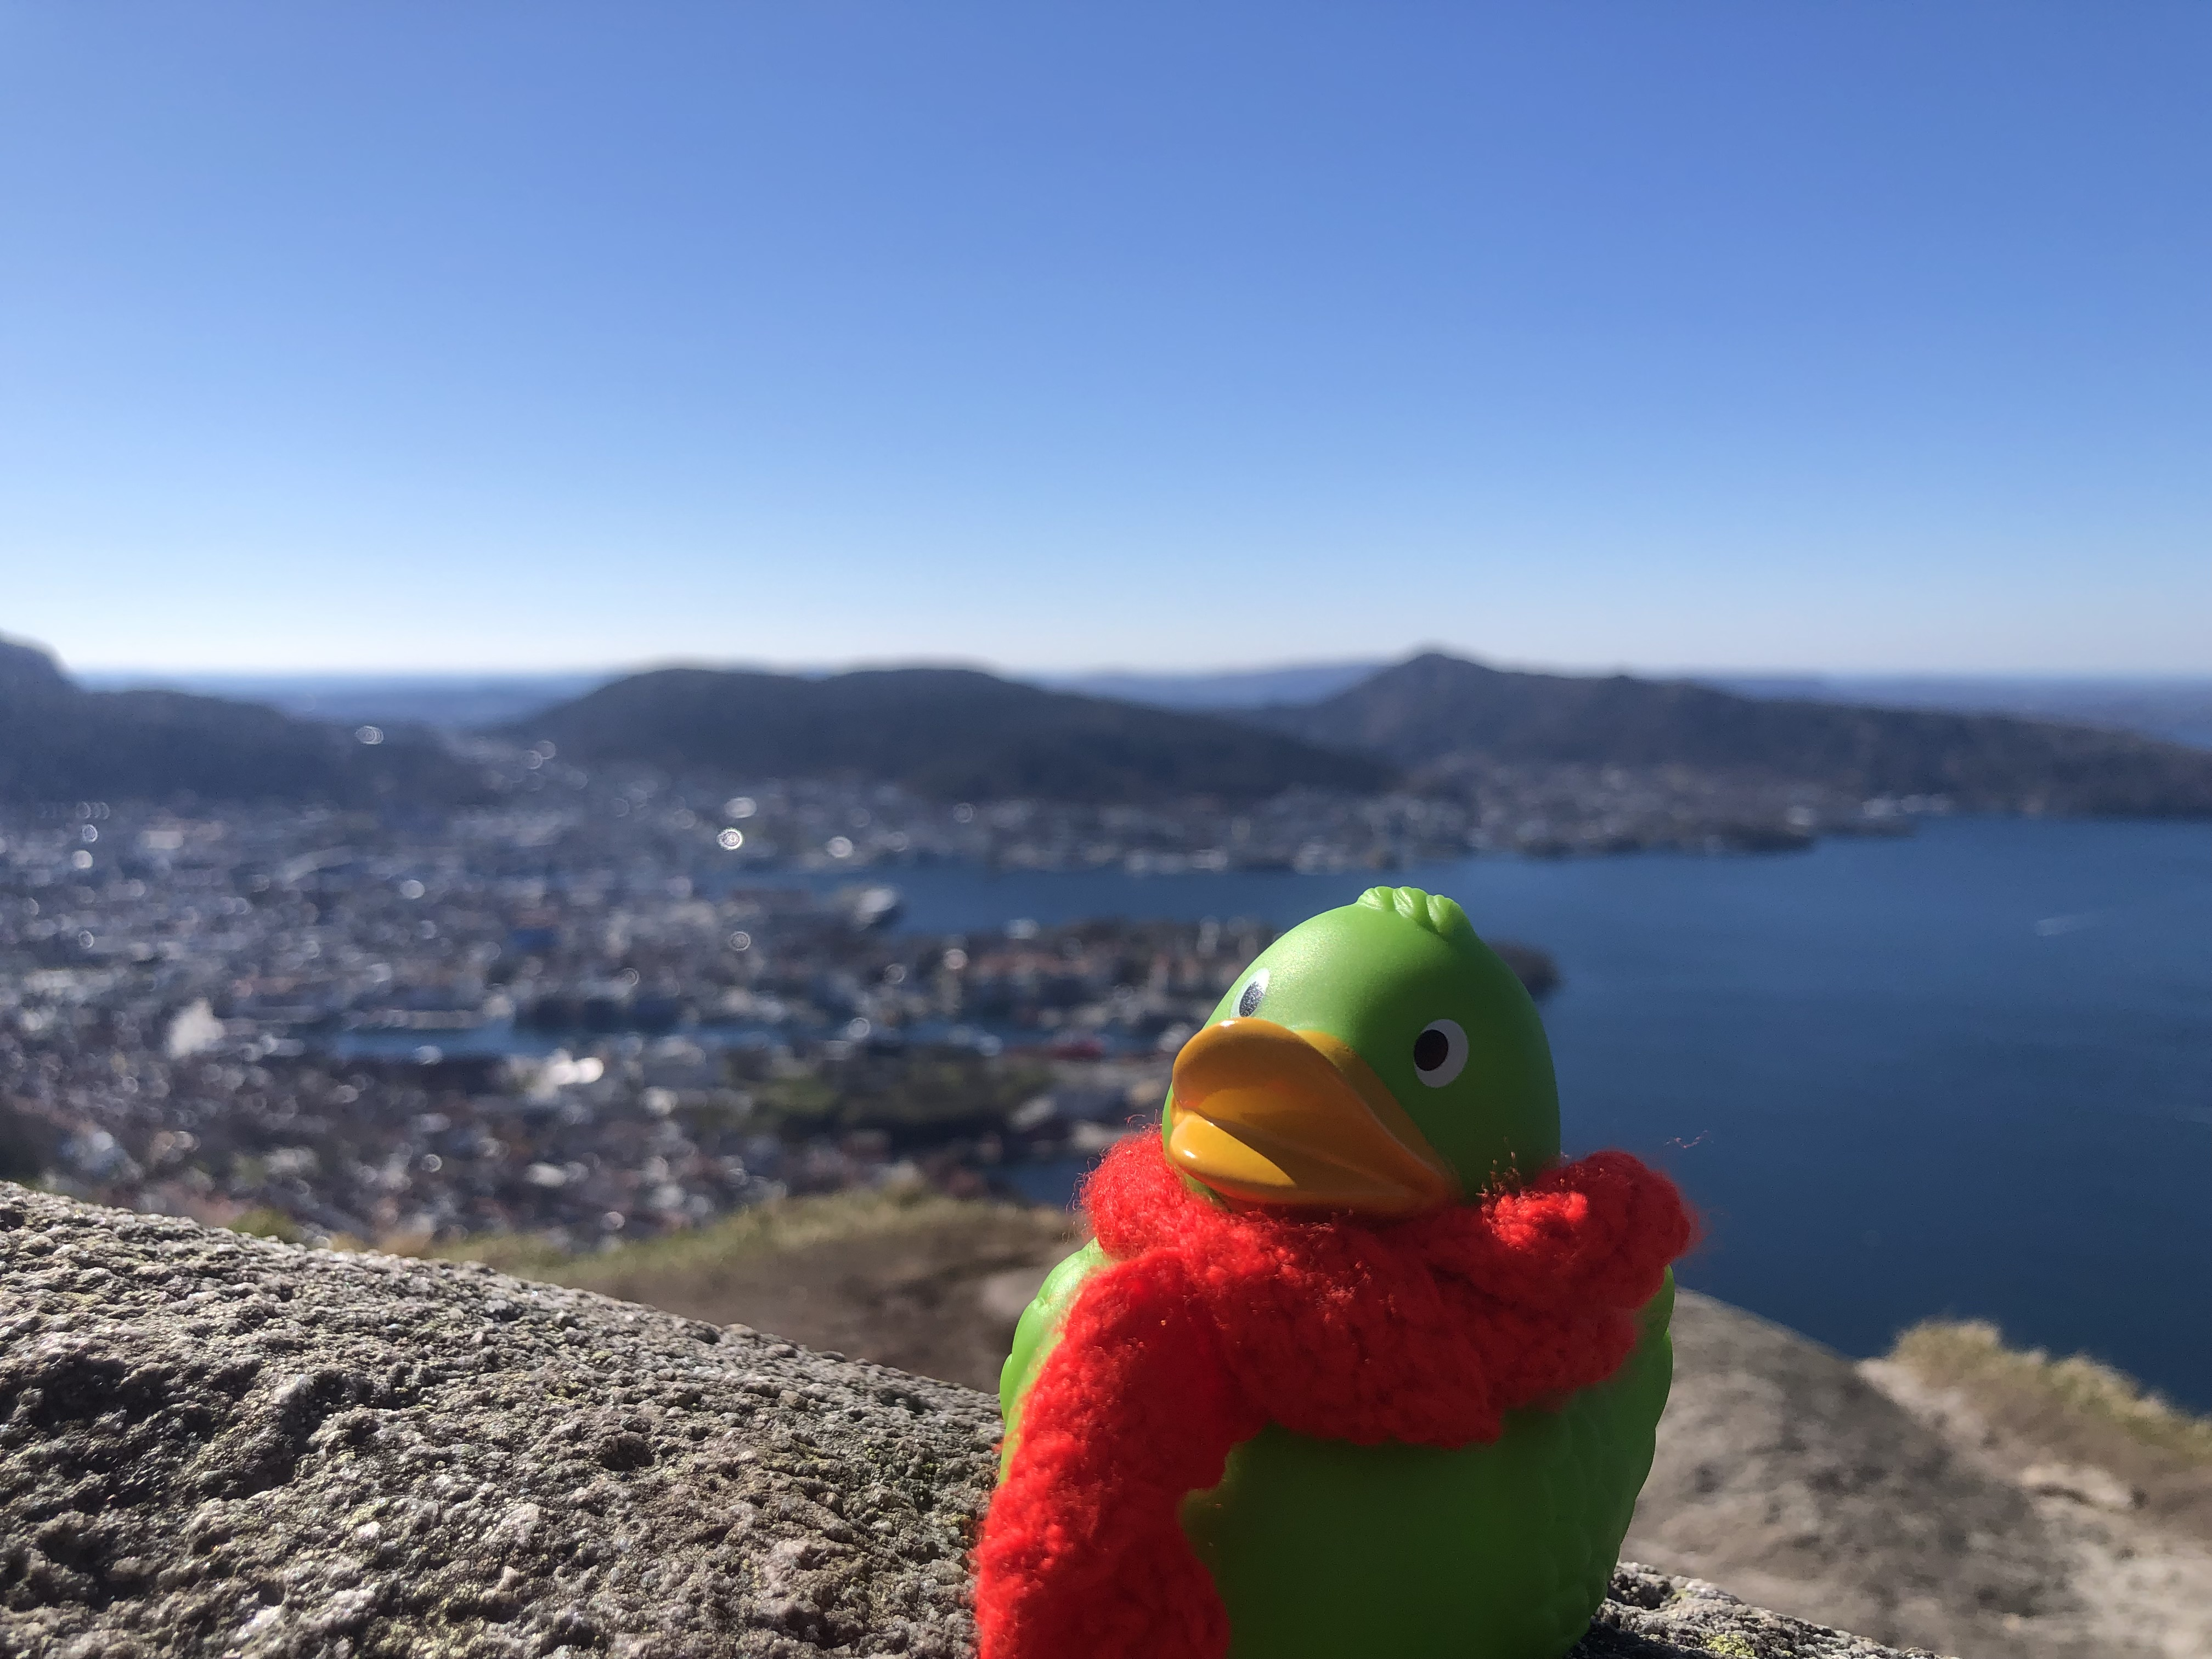
\includegraphics[height = 4.9cm]{images/guillaume1.jpg}
        \caption{Guillaume på Sandviksfjellet}
        \label{fig:guillaume1}
    \end{figure}
\end{frame}

\section{Relasjonsalgebra}
\subsection*{Operatorer}
\begin{frame}{Operatorer}
\begin{tabular}{l|l|l}
 Operator & Betydning & Eksempel\\\hline
 $\pi_{columns}(Tabell)$ & Projection (SELECT DISTINCT) & $\pi_{title, year}(Film)$\\\pause
 $\sigma_{condition}(Tabell)$ & Condition (WHERE) & $\sigma_{year > 2015}(Film)$\\\pause
 $A \times B$ & Cross join / Cartesian product & $Film \times Screening$\\\pause
 $A \cap B$ & Intersection & $Film1 \cap Film2$ \\\pause
 $A \cup B$ & Union & $Film1 \cup Film2$ \\\pause
 $A \setminus B$ & Set difference &  $Film1 \setminus Film2$\\\pause
 $A \bowtie_{condition} B$ & Inner Join & $A \bowtie_{{film\_id}={film\_id}} B$
\end{tabular}
\end{frame}

\subsection*{Eksempler}
\begin{frame}[fragile]{Eksempel 1}
\begin{minted}{sql}
SELECT DISTINCT Country
FROM Film
WHERE year < 1950
\end{minted}
\pause
$\pi_{Country}\textcolor{blue}{(}\sigma_{year < 1950}\textcolor{red}{(}Film\textcolor{red}{)}\textcolor{blue}{)}$
\end{frame}

\begin{frame}[fragile]{Eksempel 2}
\begin{minted}{sql}
SELECT DISTINCT title, year
FROM Film, Director
WHERE Film.dir_id = Director.id
AND Film.year = 1992
\end{minted}
\pause
$\pi_{title, year}\textcolor{blue}{(}\sigma_{year = 1992}\textcolor{red}{(}Film\textcolor{red}{)} \bowtie_{Film.dir\_id=Director.id}\textcolor{red}{(}Director\textcolor{red}{)}\textcolor{blue}{)}$
\end{frame}

\begin{frame}[fragile]{Eksempel 3}
\begin{minted}{sql}
SELECT Country.name, capital, inhabitants
FROM Country, City
WHERE Country.capital = City.id
AND inhabitants < 500000
\end{minted}
\pause
$\pi_{Country.name, capital, inhabitants}\textcolor{blue}{(}\sigma_{inhabitants < 500000}\textcolor{green}{(}\textcolor{red}{(}Country\textcolor{red}{)}\bowtie_{Capital=City.id}\textcolor{red}{(}City\textcolor{red}{)}\textcolor{green}{)}\textcolor{blue}{)}$
\end{frame}

\subsection*{Spørretid}
\begin{frame}{Spørsmål?}
    \begin{figure}
        \centering
        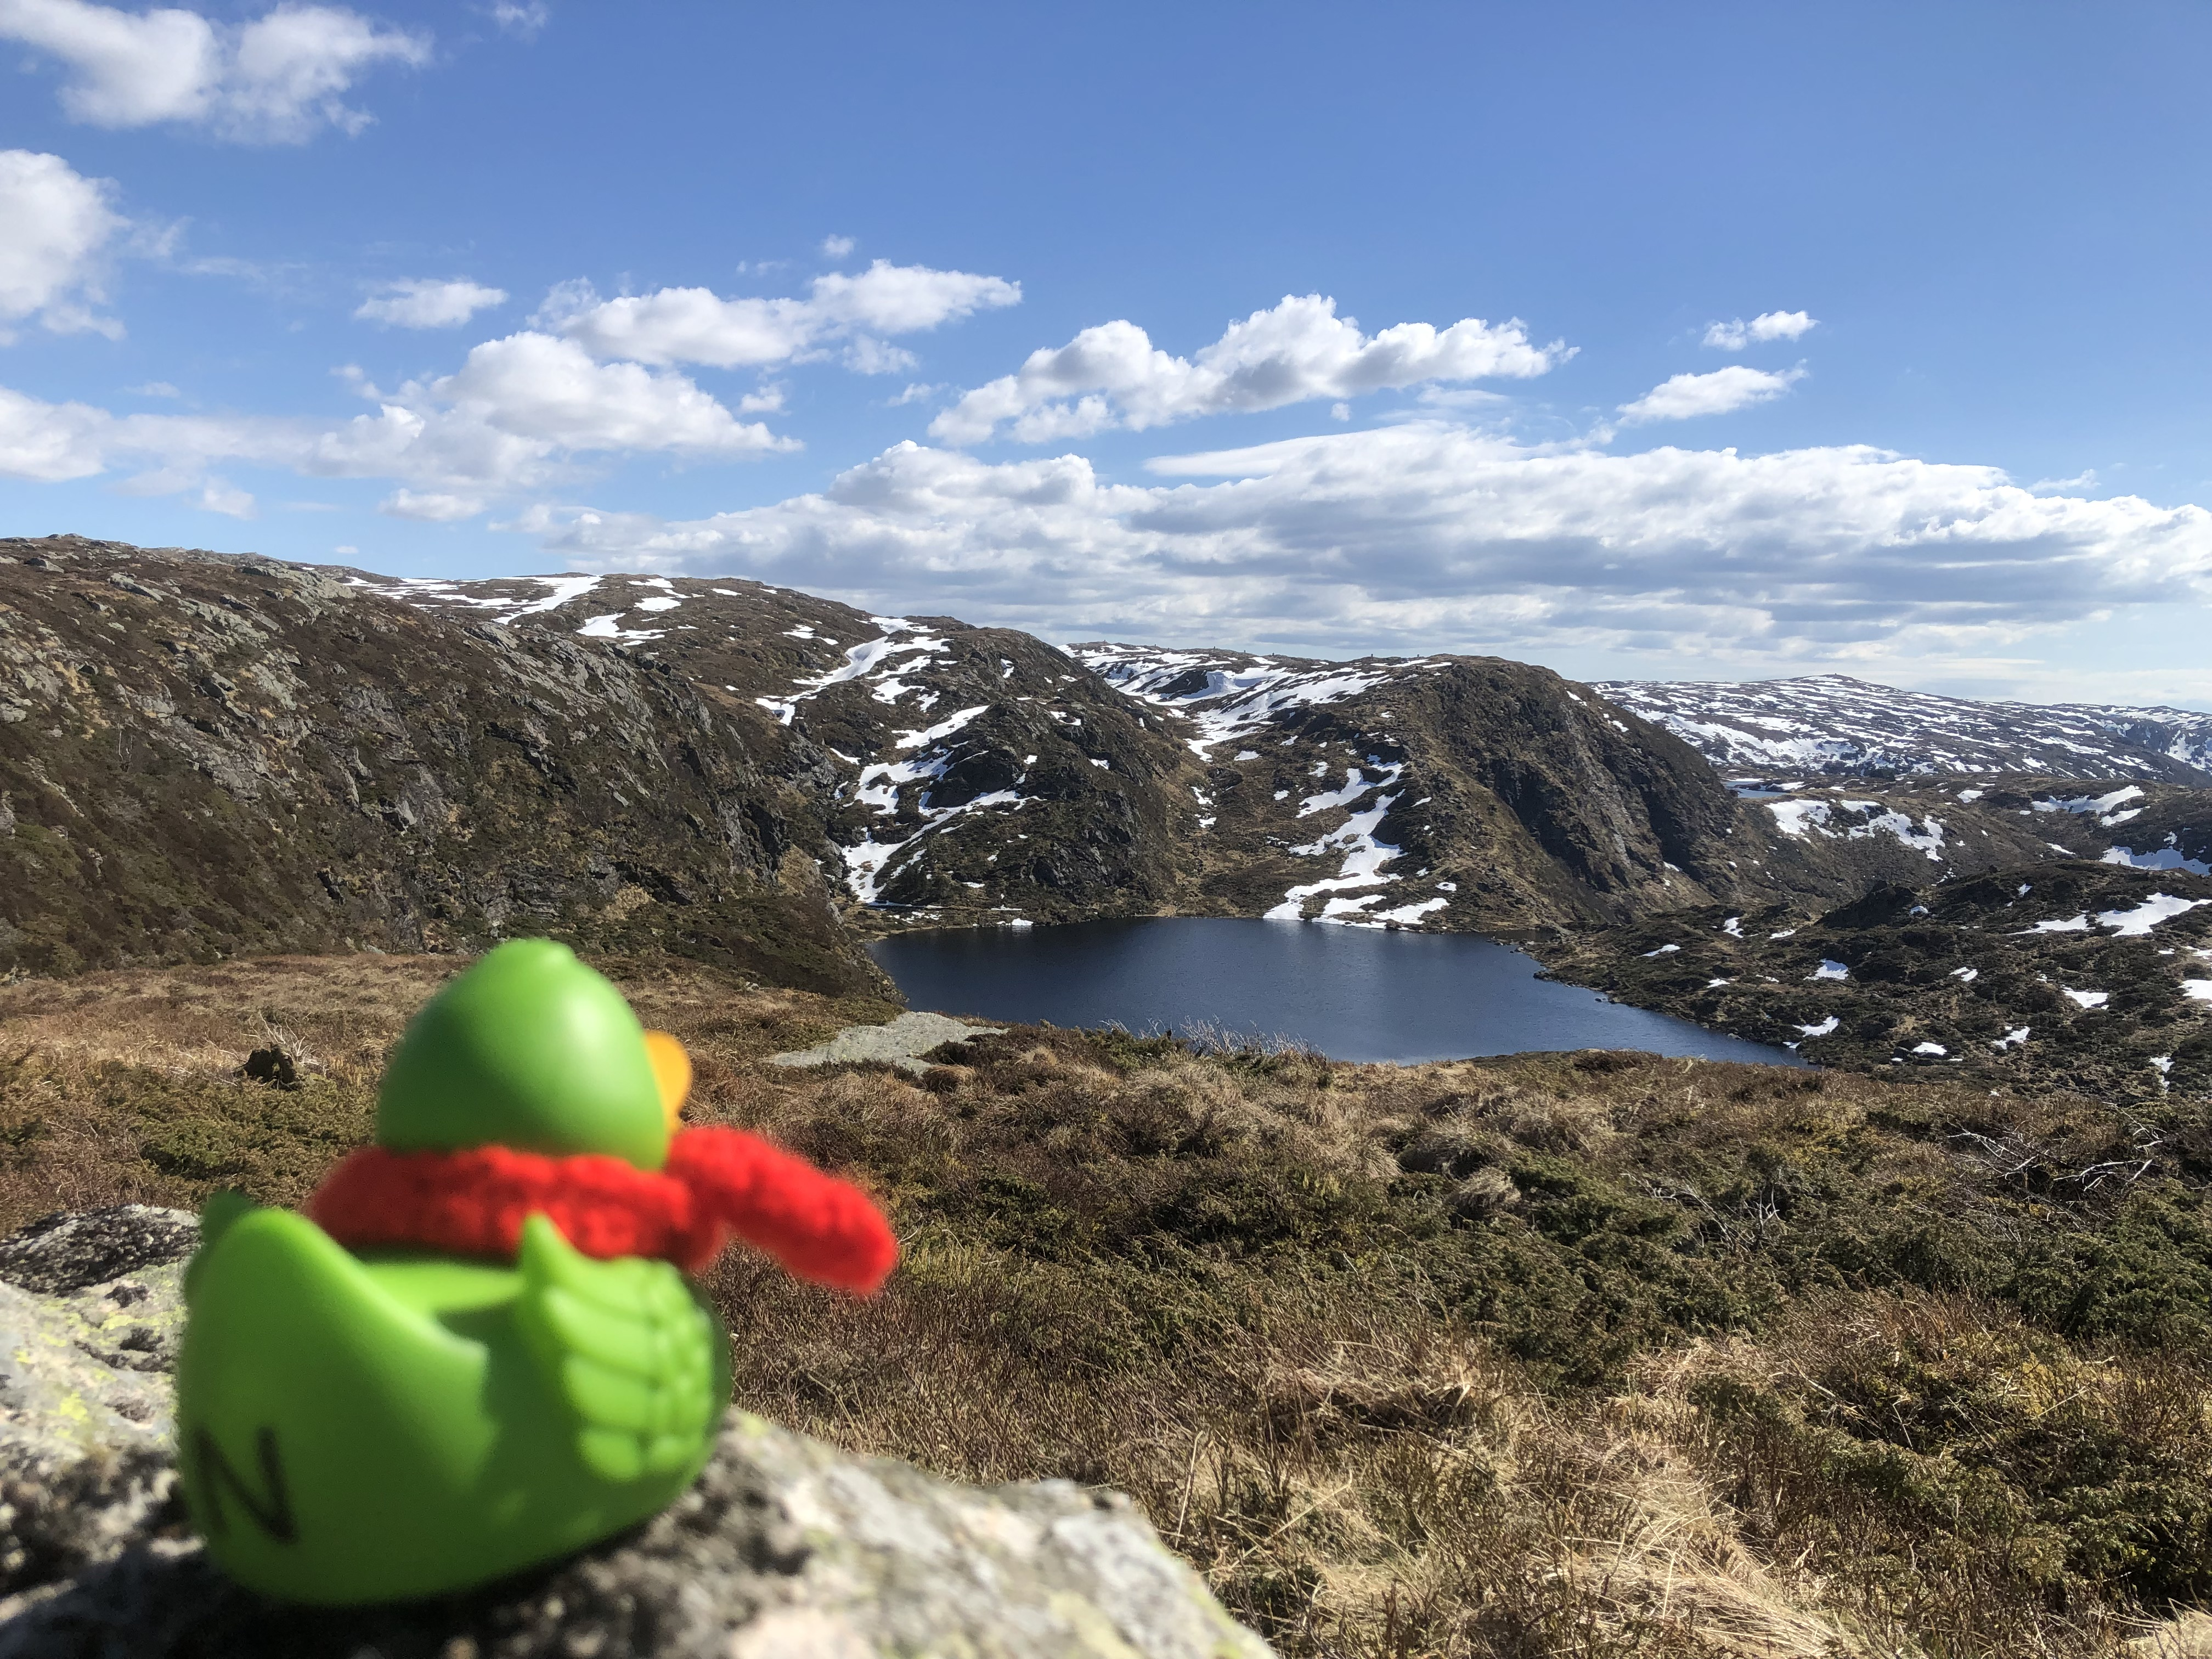
\includegraphics[height = 4.9cm]{images/guillaume4.jpg}
        \caption{Guillaume på Vidden}
        \label{fig:guillaume4}
    \end{figure}
\end{frame}
\section{ER-Diagrammer}
\begin{frame}{Entity-Relationship Diagrammer}
    \begin{itemize}[<+->]
        \item Grafisk versjon av en database
        \item Identifikasjon av entiteter
        \item Identifikasjon av sammenheng mellom entiteter
    \end{itemize}
\end{frame}

\subsection*{Kardinalitet}
\begin{frame}{Kardinalitet}
\begin{columns}
    \begin{column}{0.48\textwidth}
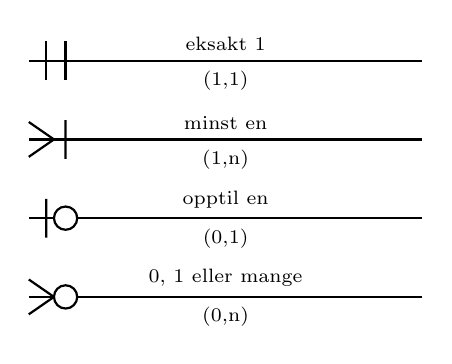
\begin{tikzpicture}[every node/.style={font=\scriptsize}]
    \draw[mone-,thick] (0,0) -- node[above]{eksakt 1}node[below]{(1,1)} (5,0);
    \draw[mmany-,thick] (0,-1) -- node[above]{minst en}node[below]{(1,n)} (5,-1);
    \draw[oone-,thick] (0,-2) -- node[above]{opptil en}node[below]{(0,1)} (5,-2);
    \draw[omany-,thick] (0,-3) -- node[above]{ 0, 1 eller mange}node[below]{(0,n)} (5,-3);
    \end{tikzpicture}
 	\end{column}
    \begin{column}{0.48\textwidth}
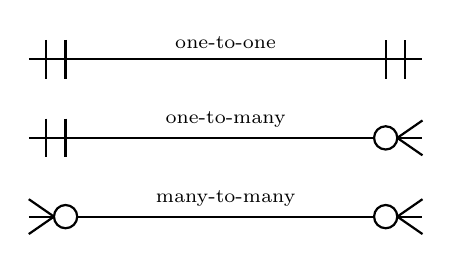
\begin{tikzpicture}[every node/.style={font=\scriptsize}]
    \draw[mone-mone,thick] (0,0) -- node[above]{one-to-one}node[below]{} (5,0);
    \draw[mone-omany,thick] (0,-1) -- node[above]{one-to-many}node[below]{} (5,-1);
    \draw[omany-omany,thick] (0,-2) -- node[above]{many-to-many}node[below]{} (5,-2);
    \end{tikzpicture}
 	\end{column}
\end{columns}
    
\end{frame}

\begin{frame}{Eksempler}
    %\begin{itemize}
        %\item<1-1> Person - Fødselsby
        %\item<2-> Person (0,n) - (1,1) Fødselsby
        %\item<3-3> Kunde - Produkt
        %\item<4-> Kunde (0,n) - (0,n) Produkt
        %\item<5-5> Medarbeider - Prosjekt
        %\item<6-> Medarbeider (1,n) - (1,1) Prosjekt
        %\item<7-7> Land - Hovedstad
        %\item<8-> Land (1,1) - (1,1) Hovedstad
        %\item<9-9> Film - Regissør
        %\item<10-> Film (0,n) - (1,n) Regissør
        
    %\end{itemize}
\begin{tabular}{l|l|l}
    Tabell & Kardinalitet & Navn\\\hline\pause
    Person - Fødselsby\pause & (0,n) - (1,1) & one-to-many\\\pause
    Kunde - Produkt\pause & (0,n) - (0,n) & many-to-many\\\pause
    Medarbeider - Prosjekt\pause & (1,n) - (1,1) & one-to-many\\\pause
    Land - Hovedstad\pause & (1,1) - (1,1) & one-to-one\\\pause
    Film - Regissør\pause & (0,n) - (1,n) & many-to-many
    \end{tabular}
\end{frame}

\begin{frame}{}
    \begin{figure}
        \centering
        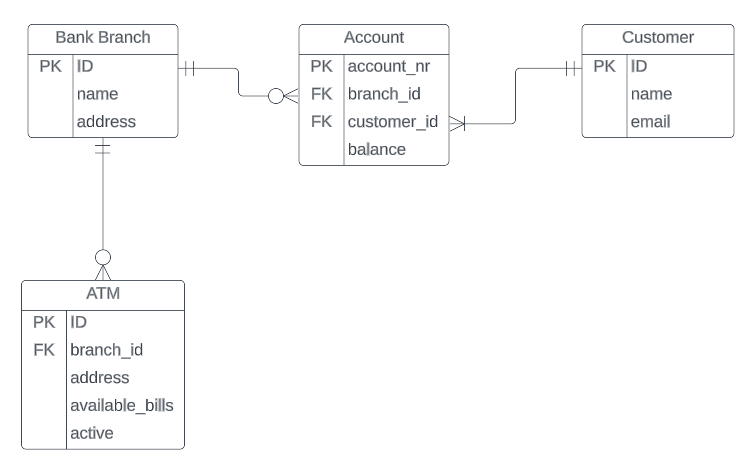
\includegraphics[height = 4.9cm]{images/erdiagram.png}
        \caption{Eksempel ER-diagram fra oblig 2}
        \label{fig:erdiagram}
    \end{figure}
\end{frame}

\subsection*{Spørretid}
\begin{frame}{Spørsmål?}
    \begin{figure}
        \centering
        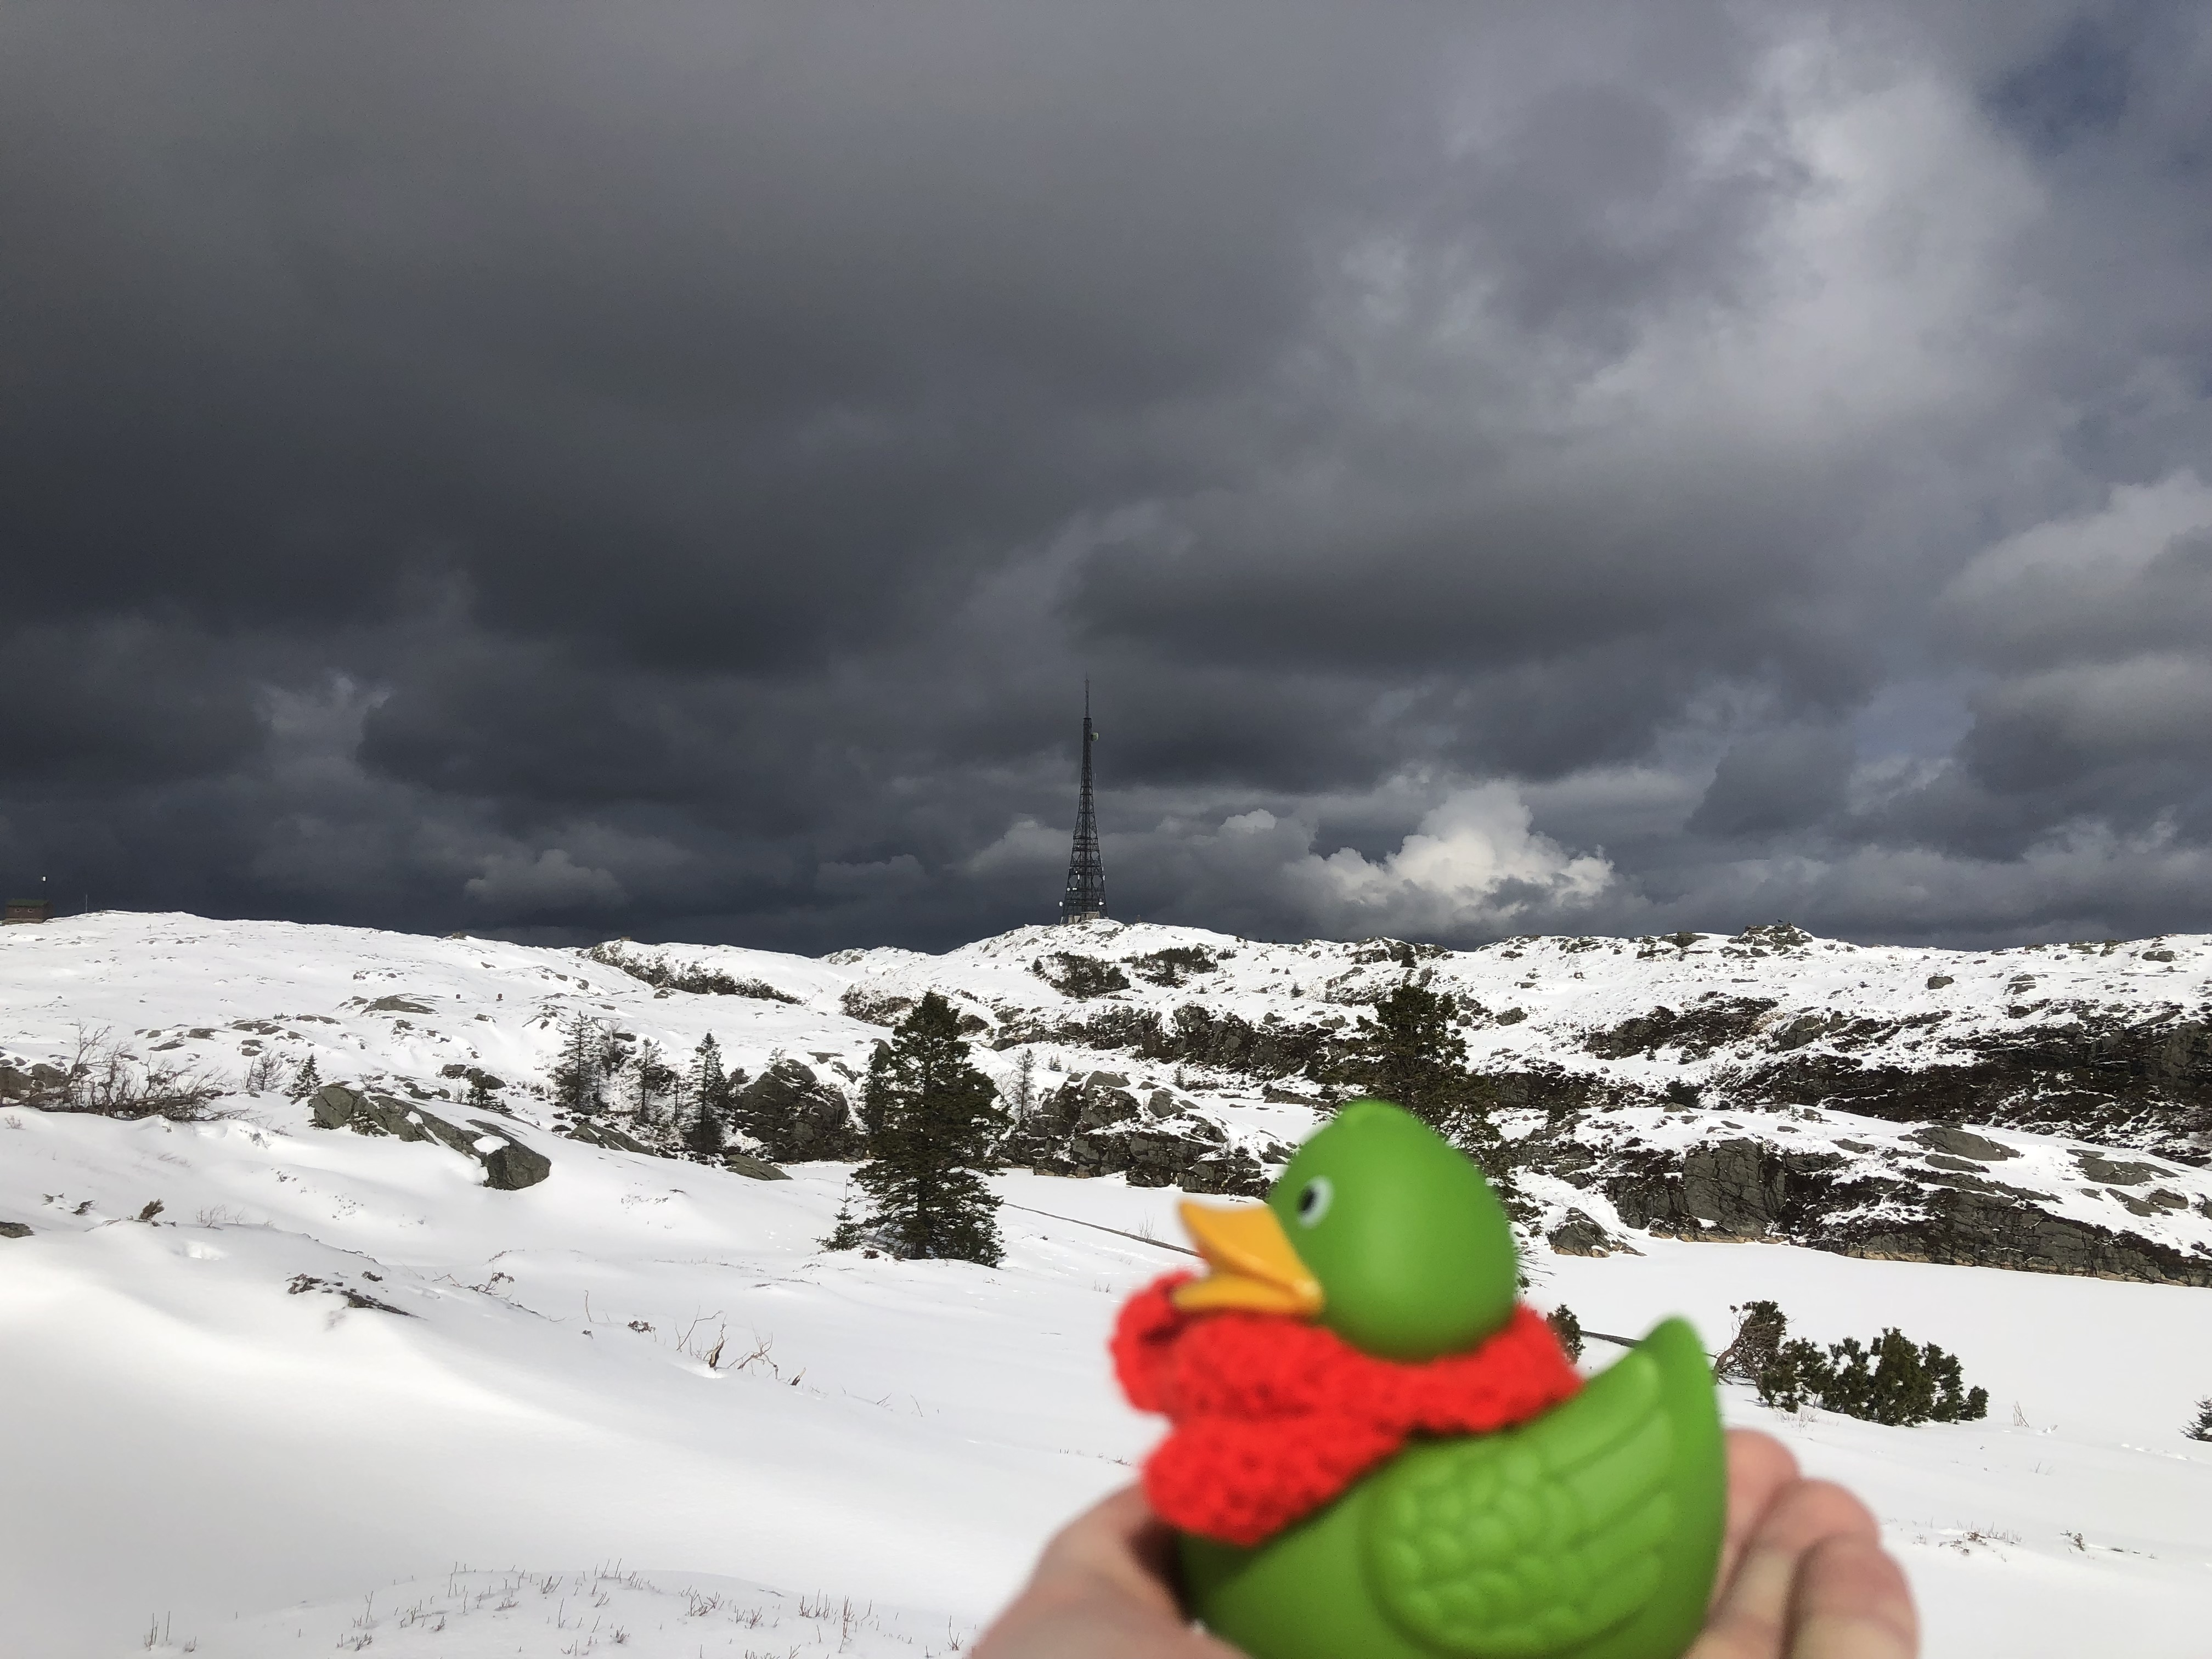
\includegraphics[height = 4.9cm]{images/guillaume6.jpg}
        \caption{Guillaume på Blåmanen}
        \label{fig:guillaume6}
    \end{figure}
\end{frame}
\section{Normalisasjon}
\subsection*{Hvorfor gjør man normalisasjon?}
\begin{frame}{Hvorfor normalisasjon?}
\begin{itemize}[<+->]
    \item Unngå redundante informasjoner
    \item Bedre å oppdatere informasjoner hvis de bare finnes en gang
    \item Lettere å bruke en stor database
    \item Visualisering av en database
\end{itemize}
\end{frame}

\subsection*{Viktige begrep}
\begin{frame}{Begrep}
\begin{itemize}[<+->]
    \item \textbf{Entitet: }En tabell i databasen
    \item \textbf{Attributt: }En kolonne i en tabell
    \item \textbf{Nøkkel: }En kolonne som bestemmer verdier i en/noen flere kolonner 
    \item \textbf{Supernøkkel: }En nøkkel som bestemmer verdier i alle andre kolonnene 
    \item \textbf{Kandidatnøkkel: }En minimal supernøkkel
\end{itemize}
\end{frame}

\begin{frame}{Functional Dependencies}
\begin{itemize}[<+->]
    \item En eller flere kolonner bestemmer verdier av andre kolonner
    \item $A \rightarrow B$ (A bestemmer B)
    \item $A,B \rightarrow C, D, E$ (A og B bestemmer C, D og E)
    \item PersonNr $\rightarrow$ Navn (det samme nummeret er den samme personen)
    \item ZipCode $\rightarrow$ City (den samme postkoden er den samme byen)
\end{itemize}
\end{frame}

\subsection*{Anomalier}
\begin{frame}{Eksempel}
%\begin{center}
\begin{tabular}{l|l|l|l|l}
 StudentNr & Name & Address & KursNr & KursName \\\hline
 580 & Ola NordmaNN & 5075 Bergen Fv14 & INF237 & Algoritme Engineering\\
 580 & Ola NordmaNN & 5075 Bergen Fv14 & INF273 & Meta Heuristikker\\
 580 & Ola NordmaNN & 5075 Bergen Fv14 & INF227 & Logikk\\
 256 & Max MustermaNN & 5055 Bergen Lv85 & INF237 & Algoritme Engineering\\
\end{tabular}
\\[5mm]
Hva er problemet her?\\\pause
Informasjoner blir lagret dobbelt.\\
Hvis kursnavn eller studentadressen endrer seg, må den endres flere ganger.
%\end{center}
\end{frame}

\begin{frame}{Anomalier}
\begin{itemize}[<+->]
    \item \textbf{Insertion Anomaly:} Den samme informasjonen blir lagt inn med andre verdier
    \item \textbf{Update Anomaly:} Dobbel informasjon blir ikke oppdatert overalt
    \item \textbf{Deletion Anomaly}: Data forsvinner fordi den ikke finnes i en egen tabell
\end{itemize}

\pause

\medskip

Eksempler:
\begin{itemize}[<+->]
    \item \textbf{Insertion Anomaly:} Studenten tar et kurs til, men har nå en annen adresse 
    \item \textbf{Update Anomaly:} Kursnavnet blir oppdatert, men ikke for alle studenter
    \item \textbf{Deletion Anomaly:} En student melder seg ut av alle kurser, så forsvinner han i hele databasen
\end{itemize}
\end{frame}

\begin{frame}{Hvordan løser man problemene?}
\begin{tabular}{l|l|l}
 StudentNr & Name & Address\\\hline
 580 & Ola NordmaNN & 5075 Bergen Fv 14\\
 256 & Max MustermaNN & 5055 Bergen Lv 85\\
\end{tabular}
\vfill
\begin{tabular}{l|l}
KursNr & KursName \\\hline
INF237 & Algorithm Engineering\\
INF273 & Meta Heuristikker\\
INF227 & Logikk\\
\end{tabular}
\hfill
\begin{tabular}{l|l}
 StudentNr & KursNr\\\hline
 580 & INF237\\
 580 & INF273\\
 580 & INF227\\
 256 & INF237\\
\end{tabular}
\end{frame}

\subsection*{Normalformer}
\begin{frame}{1. Normalform (1NF)}
    \begin{block}{1. Normalform}
    Hvert attributt (kolonne) må være atomar, den kan ikke ha flere verdier (lister etc. er forbud).
    \end{block}
    \vfill
    \pause
    \begin{tabular}{l|l}
     StudentNr & KursNr\\\hline
     580 & [INF237, INF273, INF227]\\
     256 & INF237\\
     \end{tabular}
     \hfill
     \pause
     $\rightarrow$
     \hfill
     \begin{tabular}{l|l}
     StudentNr & KursNr\\\hline
     580 & INF237\\
     580 & INF273\\
     580 & INF227\\
     256 & INF237\\
    \end{tabular}
\end{frame}

\begin{frame}{2. Normalform (2NF)}
    \begin{block}{2. Normalform}
    Alle ikke-nøkkel-attributter er fullstendig funksjonell avhengig av en primærnøkkel.\\
    En ikke primær-attributt kan ikke være avhengig av bare en del av nøkkelen.
    \end{block}
    \vfill
    \only<1>{\begin{tabular}{l|l|l}
     StudentNr & KursNr & StudentNavn\\\hline
     580 & INF237 & Ola\\
     580 & INF273 & Ola\\
     580 & INF227 & Ola\\
     256 & INF237 & Max\\
     \end{tabular}
     }
     \only<2>{
     \begin{tabular}{l|l}
     StudentNr & KursNr\\\hline
     580 & INF237\\
     580 & INF273\\
     580 & INF227\\
     256 & INF237\\
    \end{tabular}
    \hfill
    \begin{tabular}{l|l}
     StudentNr & StudentNavn\\\hline
     580 & Ola\\
     580 & Ola\\
     580 & Ola\\
     256 & Max\\
    \end{tabular}
    }
\end{frame}

\begin{frame}{3. Normalform (3NF)}
\begin{block}{3. Normalform}
    Det finnes ingen transitive avhengigheter.\\
    Det finnes ikke tre attributter A, B, C der $A \rightarrow B$ og $B \rightarrow C$ gjelder.
    \end{block}
    \vfill
    \only<1>{\begin{tabular}{l|l|l}
     Universitetet & By & Land\\\hline
     UiB & Bergen & Norge\\
     HUB & Berlin & Tyskland\\
     NTNU & Trondhjem & Norge\\
     \end{tabular}
     }
     \only<2>{
     \begin{tabular}{l|l}
     Universitetet & By\\\hline
     UiB & Bergen\\
     HUB & Berlin\\
     NTNU & Trondhjem\\
    \end{tabular}
    \hfill
    \begin{tabular}{l|l}
     By & Land\\\hline
     Bergen & Norge\\
     Berlin & Tyskland\\
     Trondhjem & Norge\\
    \end{tabular}
    }
\end{frame}

\begin{frame}{Boyce–Codd Normalform (BCNF)}
\begin{block}{Boyce-Codd Normalform ($3 \frac{1}{2}$NF)}
    Det finnes ikke to overlappende kandidatnøkler. Skjer nesten aldri.
    \end{block}
    \vfill
    $Tabell(A, B, C, D)$\\
    $A,B\rightarrow C,D; $ $C\rightarrow B$\medskip
    
    \pause
    Løsning: Split opp tabellen for å fjerne syklisk avhengig:\\
    $Tabell1(A, C, D)$, $Tabell2(C, B)$\\
    $A\rightarrow C,D; $ $C\rightarrow B$\medskip
\end{frame}

\subsection*{Spørretid}
\begin{frame}{Spørsmål?}
    \begin{figure}
        \centering
        \includegraphics[height = 4.9cm]{images/guillaume9.jpg}
        \caption{Guillaume foran Tvindefossen}
        \label{fig:guillaume9}
    \end{figure}
\end{frame}

\section{Filer}
\subsection*{Alt er lagret i filer}
\begin{frame}{HDD}
    \begin{itemize}[<+->]
        \item Disk = permanent lagring
        \item Hard disk drive (HDD)
        \begin{itemize}
          \item Roterende magnetiske fat 
          \item Mekaniske bevegelser tar tid
        \end{itemize}
        \item Lese og skrive til disken krever:
        \begin{itemize}
          \item Posisjonere armene
          \item Vente for at riktig sektor passerer under armene
          \item Overføre data fra/til RAM
        \end{itemize}
    \end{itemize}
\end{frame}

\begin{frame}{SSD}
  \begin{itemize}[<+->]
    \item Solid State Disk (SSD)
    \begin{itemize}
      \item Ingen bevegelige deler
      \item Mye raskere enkelt lookup
      \item Erstatter hard disker i mange områder
    \end{itemize}
    \item Forskjellen på HDD og SSD
    \begin{itemize}
      \item SSD er raskt
      \item HDD er billig
    \end{itemize}
\end{itemize}
\end{frame}



\subsection*{Terminologi}
\begin{frame}{Terminologi}
  \begin{itemize}[<+->]
    \item Tabell   = File
    \item Rad      = Record
    \item Attributt = Field
  \end{itemize}
\end{frame}

\subsection*{Blocks}
\begin{frame}
  \begin{columns}
  \begin{column}{0.48\textwidth}
    \begin{figure}
        %\centering
        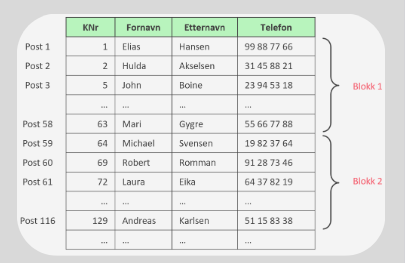
\includegraphics[height = 3.8cm]{images/blocks.png}
        \caption{En fil delt i blokker}
        \label{fig:blocks}
    \end{figure}
  \end{column}
  \begin{column}{0.48\textwidth}
    \begin{itemize}[<+->]
        \item En blokk er den minste enheten for å overføre data mellom RAM og ekstern lagring (HDD/SSD)
        \item Typisk blokk størrelse: 4KB
        \item En blokk kan generelt inneholde flere records (rader) 
    \end{itemize}
  \end{column}
  \end{columns}
\end{frame}

\subsection*{Spørretid}
\begin{frame}{Spørsmål?}
    \begin{figure}
        \centering
        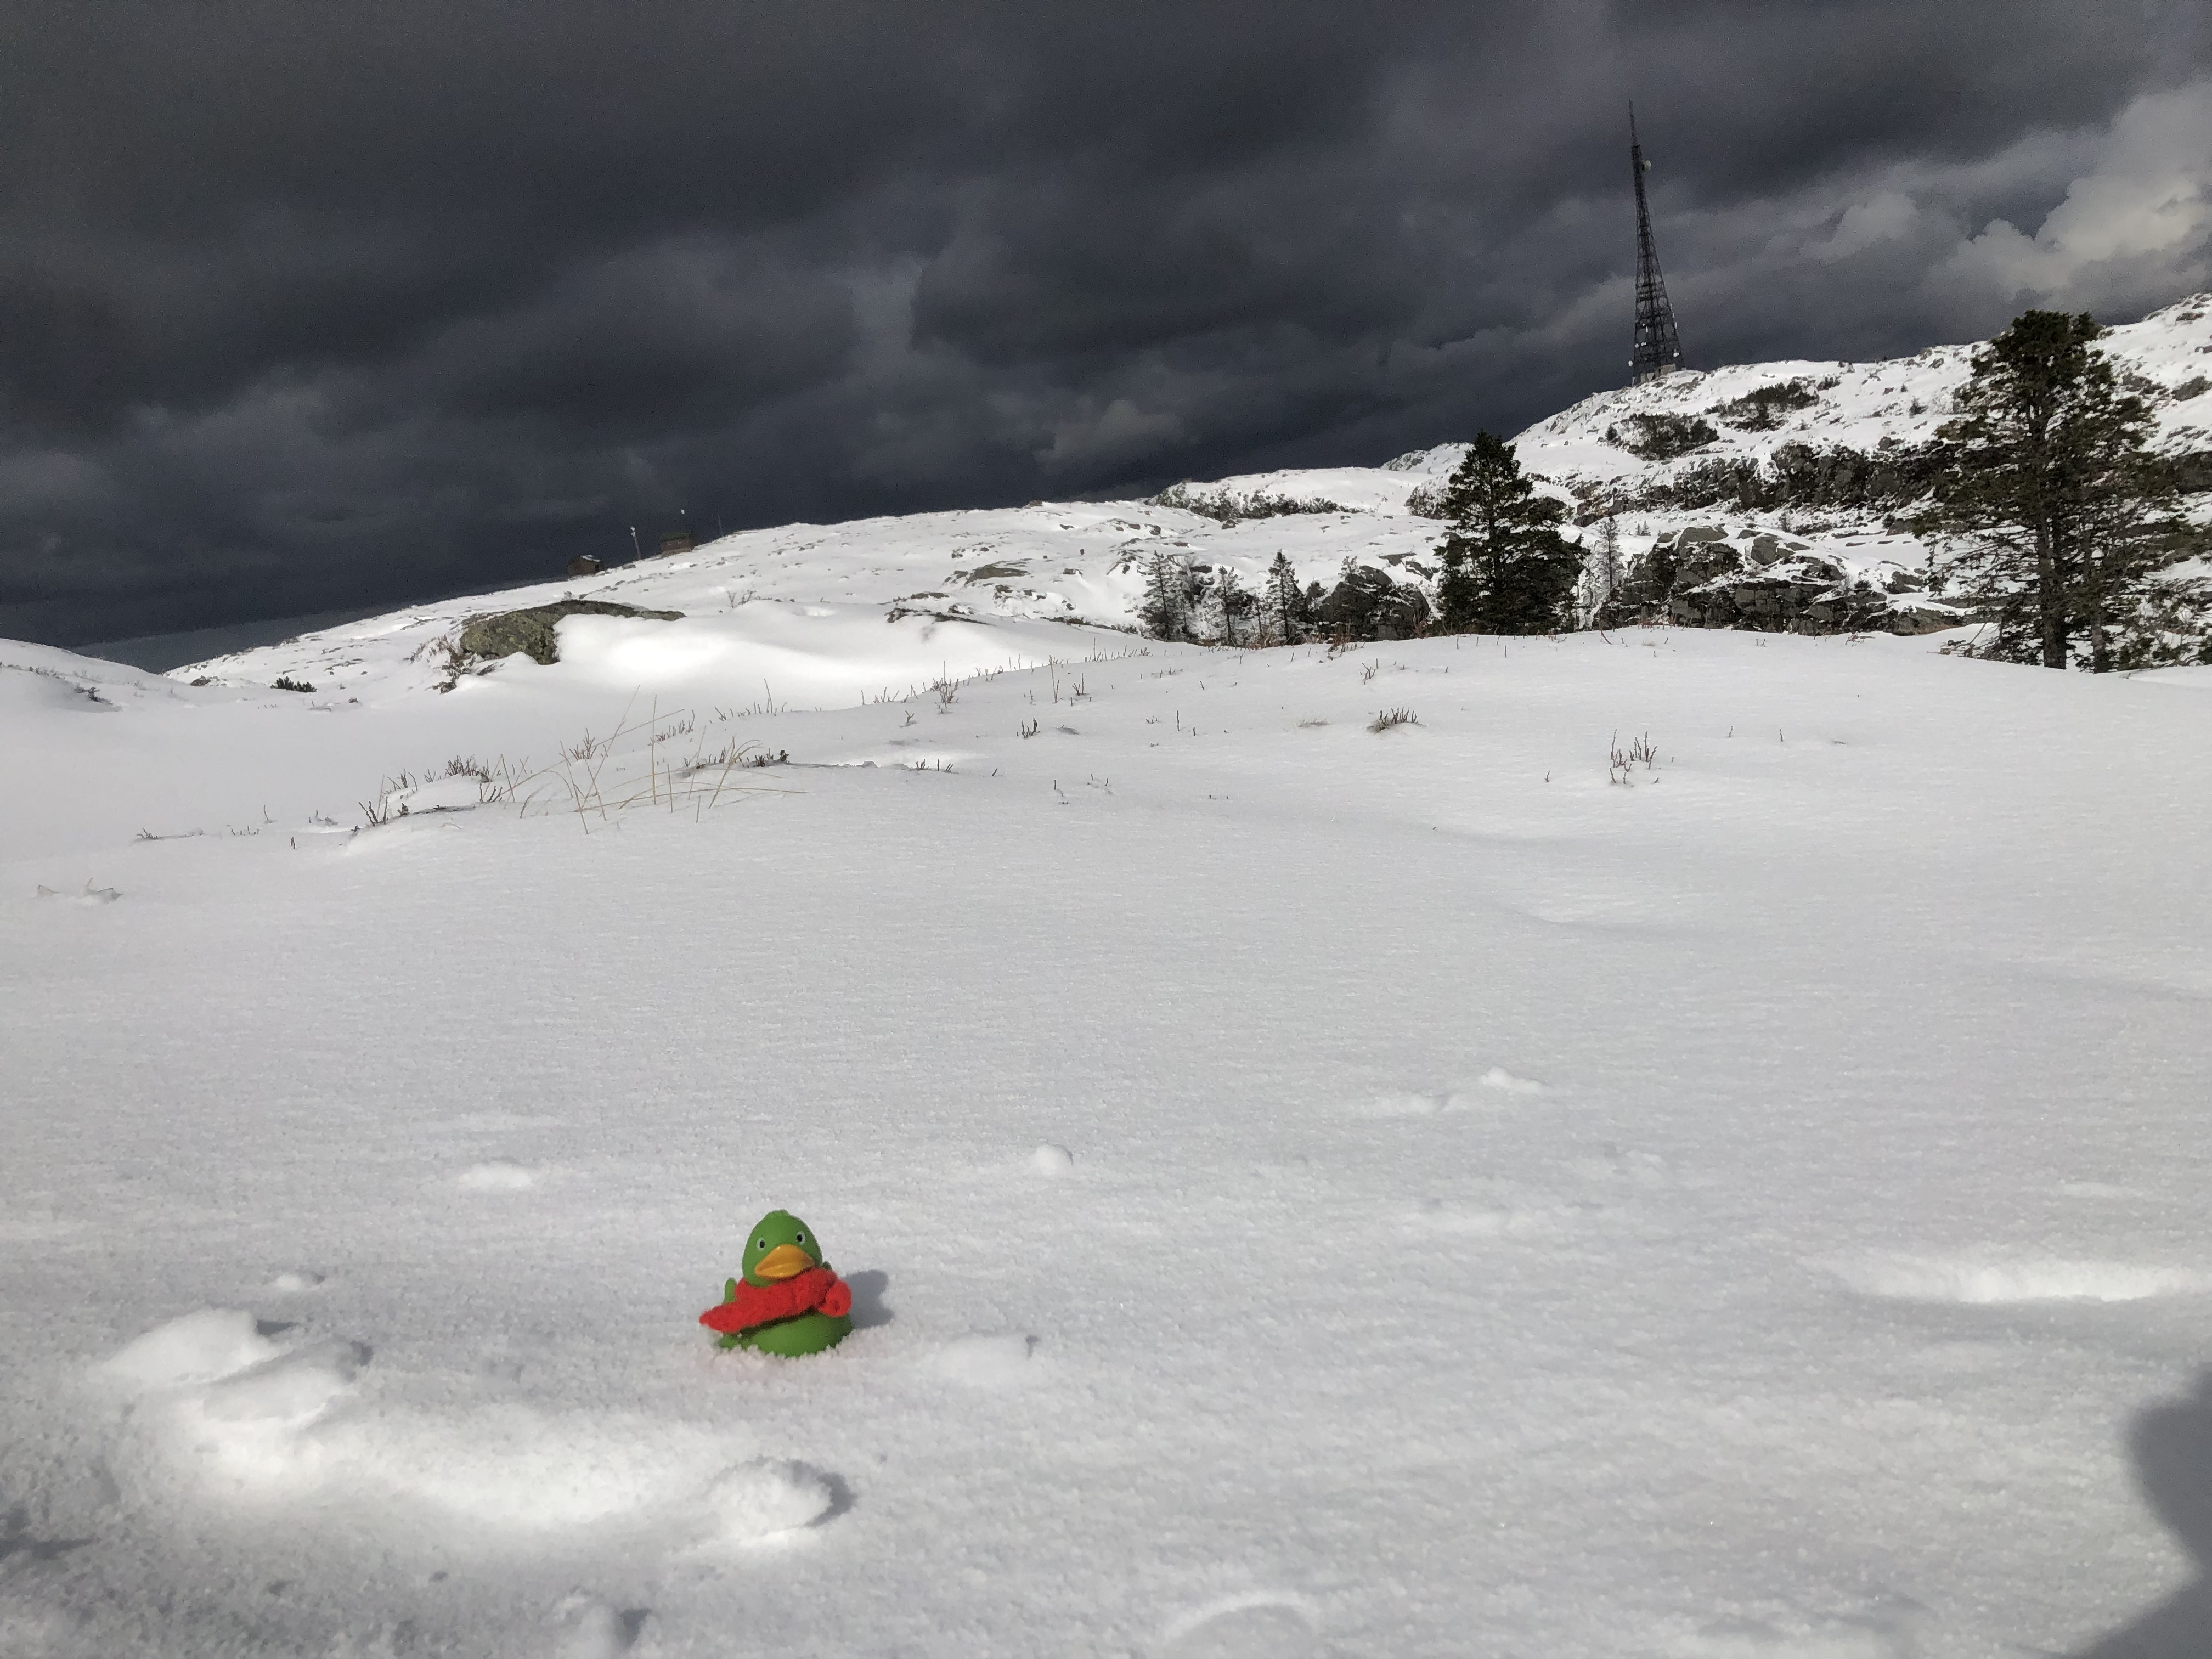
\includegraphics[height = 4.9cm]{images/guillaume7.jpg}
        \caption{Guillaume i snøen}
        \label{fig:guillaume8}
    \end{figure}
\end{frame}

\section{Indekser}
\subsection*{Hvorfor indekser?}
\begin{frame}{Indekser}
    \begin{itemize}[<+->]
        \item Rows er ikke sortert
        \item $\rightarrow$ finne informasjoner med WHERE tar tid
        \item Indekser er ekstrastrukturer som forenkler søking i tabeller
        \item Kan være en eller flere kolonner 
        \item Indekser funker som ordbok/lookup table
        \item Ulempe: De tar plass, må oppdateres
        \item Primærnøkler har automatisk en indeks på seg
        \item To typer indekser:
            \begin{itemize}
                \item B-trær
                \item Hashing
            \end{itemize}
    \end{itemize}
\end{frame}

\subsection*{B-trær}
\begin{frame}{B-trær}
    \begin{columns}
    \begin{column}{0.48\textwidth}
    \begin{figure}
        %\centering
        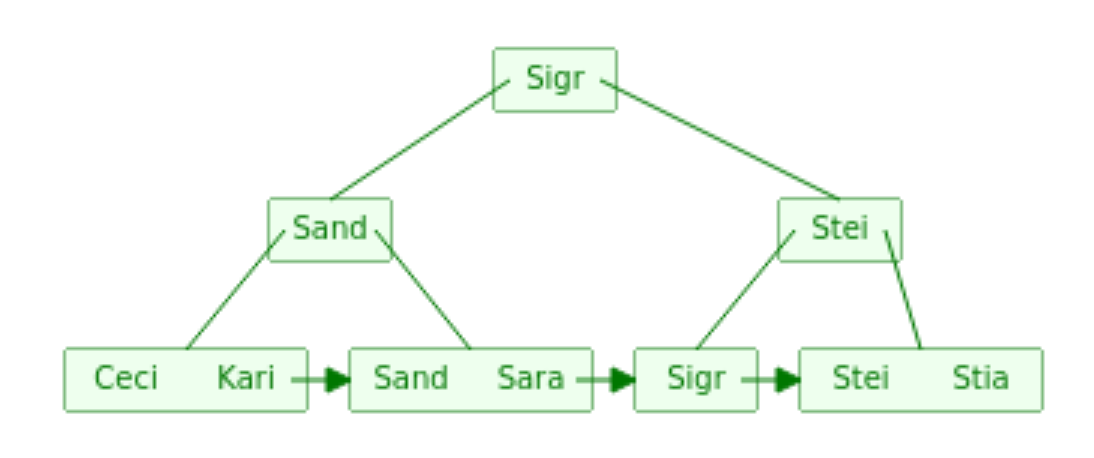
\includegraphics[height = 2.9cm]{images/btre.png}
        \caption{Eksempel B-tre}
        \label{fig:btree}
    \end{figure}
    \end{column}
    \begin{column}{0.48\textwidth}
    \begin{itemize}[<+->]
        \item Data er organisert som et søketre
        \item Alle elementer er leaves i treet 
        \item Leaves er sortert
        \item Leting etter elementer skjer gjennom graftraversal
        \item Hvis element er mindre, gå til venstre
        \item Hvis element er større, gå til høyre
        \item Kjøretiden blir $O(log(n))$ istedenfor $O(n)$
    \end{itemize}
    \end{column}
    \end{columns}
\end{frame}

\subsection*{Hashing}
\begin{frame}{Hashing}
    \begin{columns}
    \begin{column}{0.48\textwidth}
    \begin{figure}
        %\centering
        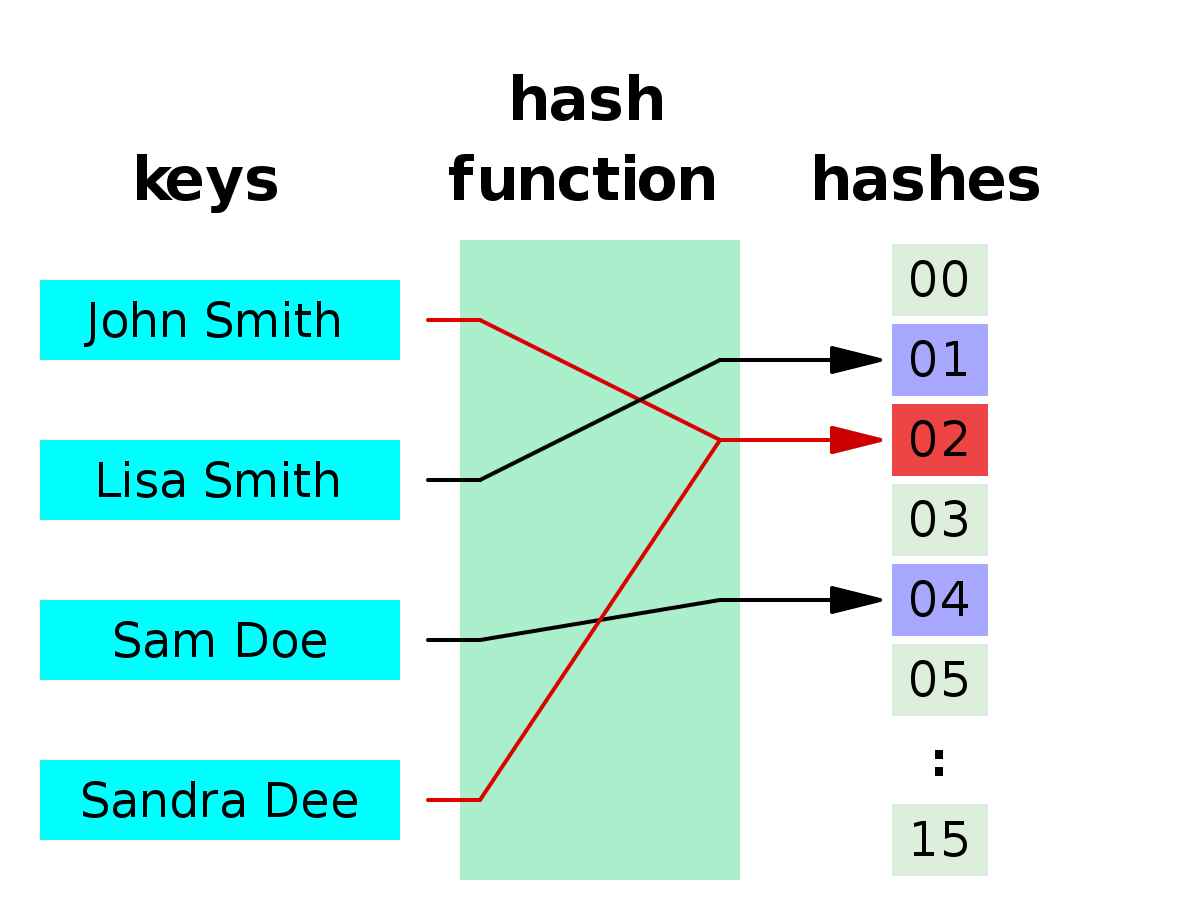
\includegraphics[height = 3.8cm]{images/hashing.png}
        \caption{Eksempel Hashing}
        \label{fig:hashing}
    \end{figure}
    \end{column}
    \begin{column}{0.48\textwidth}
    \begin{itemize}[<+->]
        \item Data blir komprimert med en engangsfunksjon
        \item Data blir lagt som liste av hashes
        \item Listen kan ikke sorteres
        \item Listeinnholdet følger ingen pattern
        \item Kjøretiden blir $O(1)$ istedenfor $O(n)$
        \item Range-Selection er drittslangsom
    \end{itemize}
    \end{column}
    \end{columns}
\end{frame}

\subsection*{Eksempel}
\begin{frame}{Hvilke indekser skulle man ha?}
    \begin{itemize}[<+->]
        \item Students(Student number*, First Name, Last Name, Gender)
        \item Indekser: Last Name,(First Name, Last Name)
        \item Staff(Staff number*, First Name, Last Name, Position)
        \item Indekser: Last Name,(First Name, Last Name), Position
        \item Course(Course Code*, Course Name, Credits)
        \item Indekser: Name? Credits?
        \item Study(Study Code*, Study name)
        \item Indekser: Study name
        \item StudyDesign(Study Code*, Course Code*, Semester Number)
        \item Indekser: Semester Number
        \item Results(Serial number*, Student number*, Grade)
        \item Indekser: Ingen?
    \end{itemize}
\end{frame}

\subsection*{Spørretid}
\begin{frame}{Spørsmål?}
    \begin{figure}
        \centering
        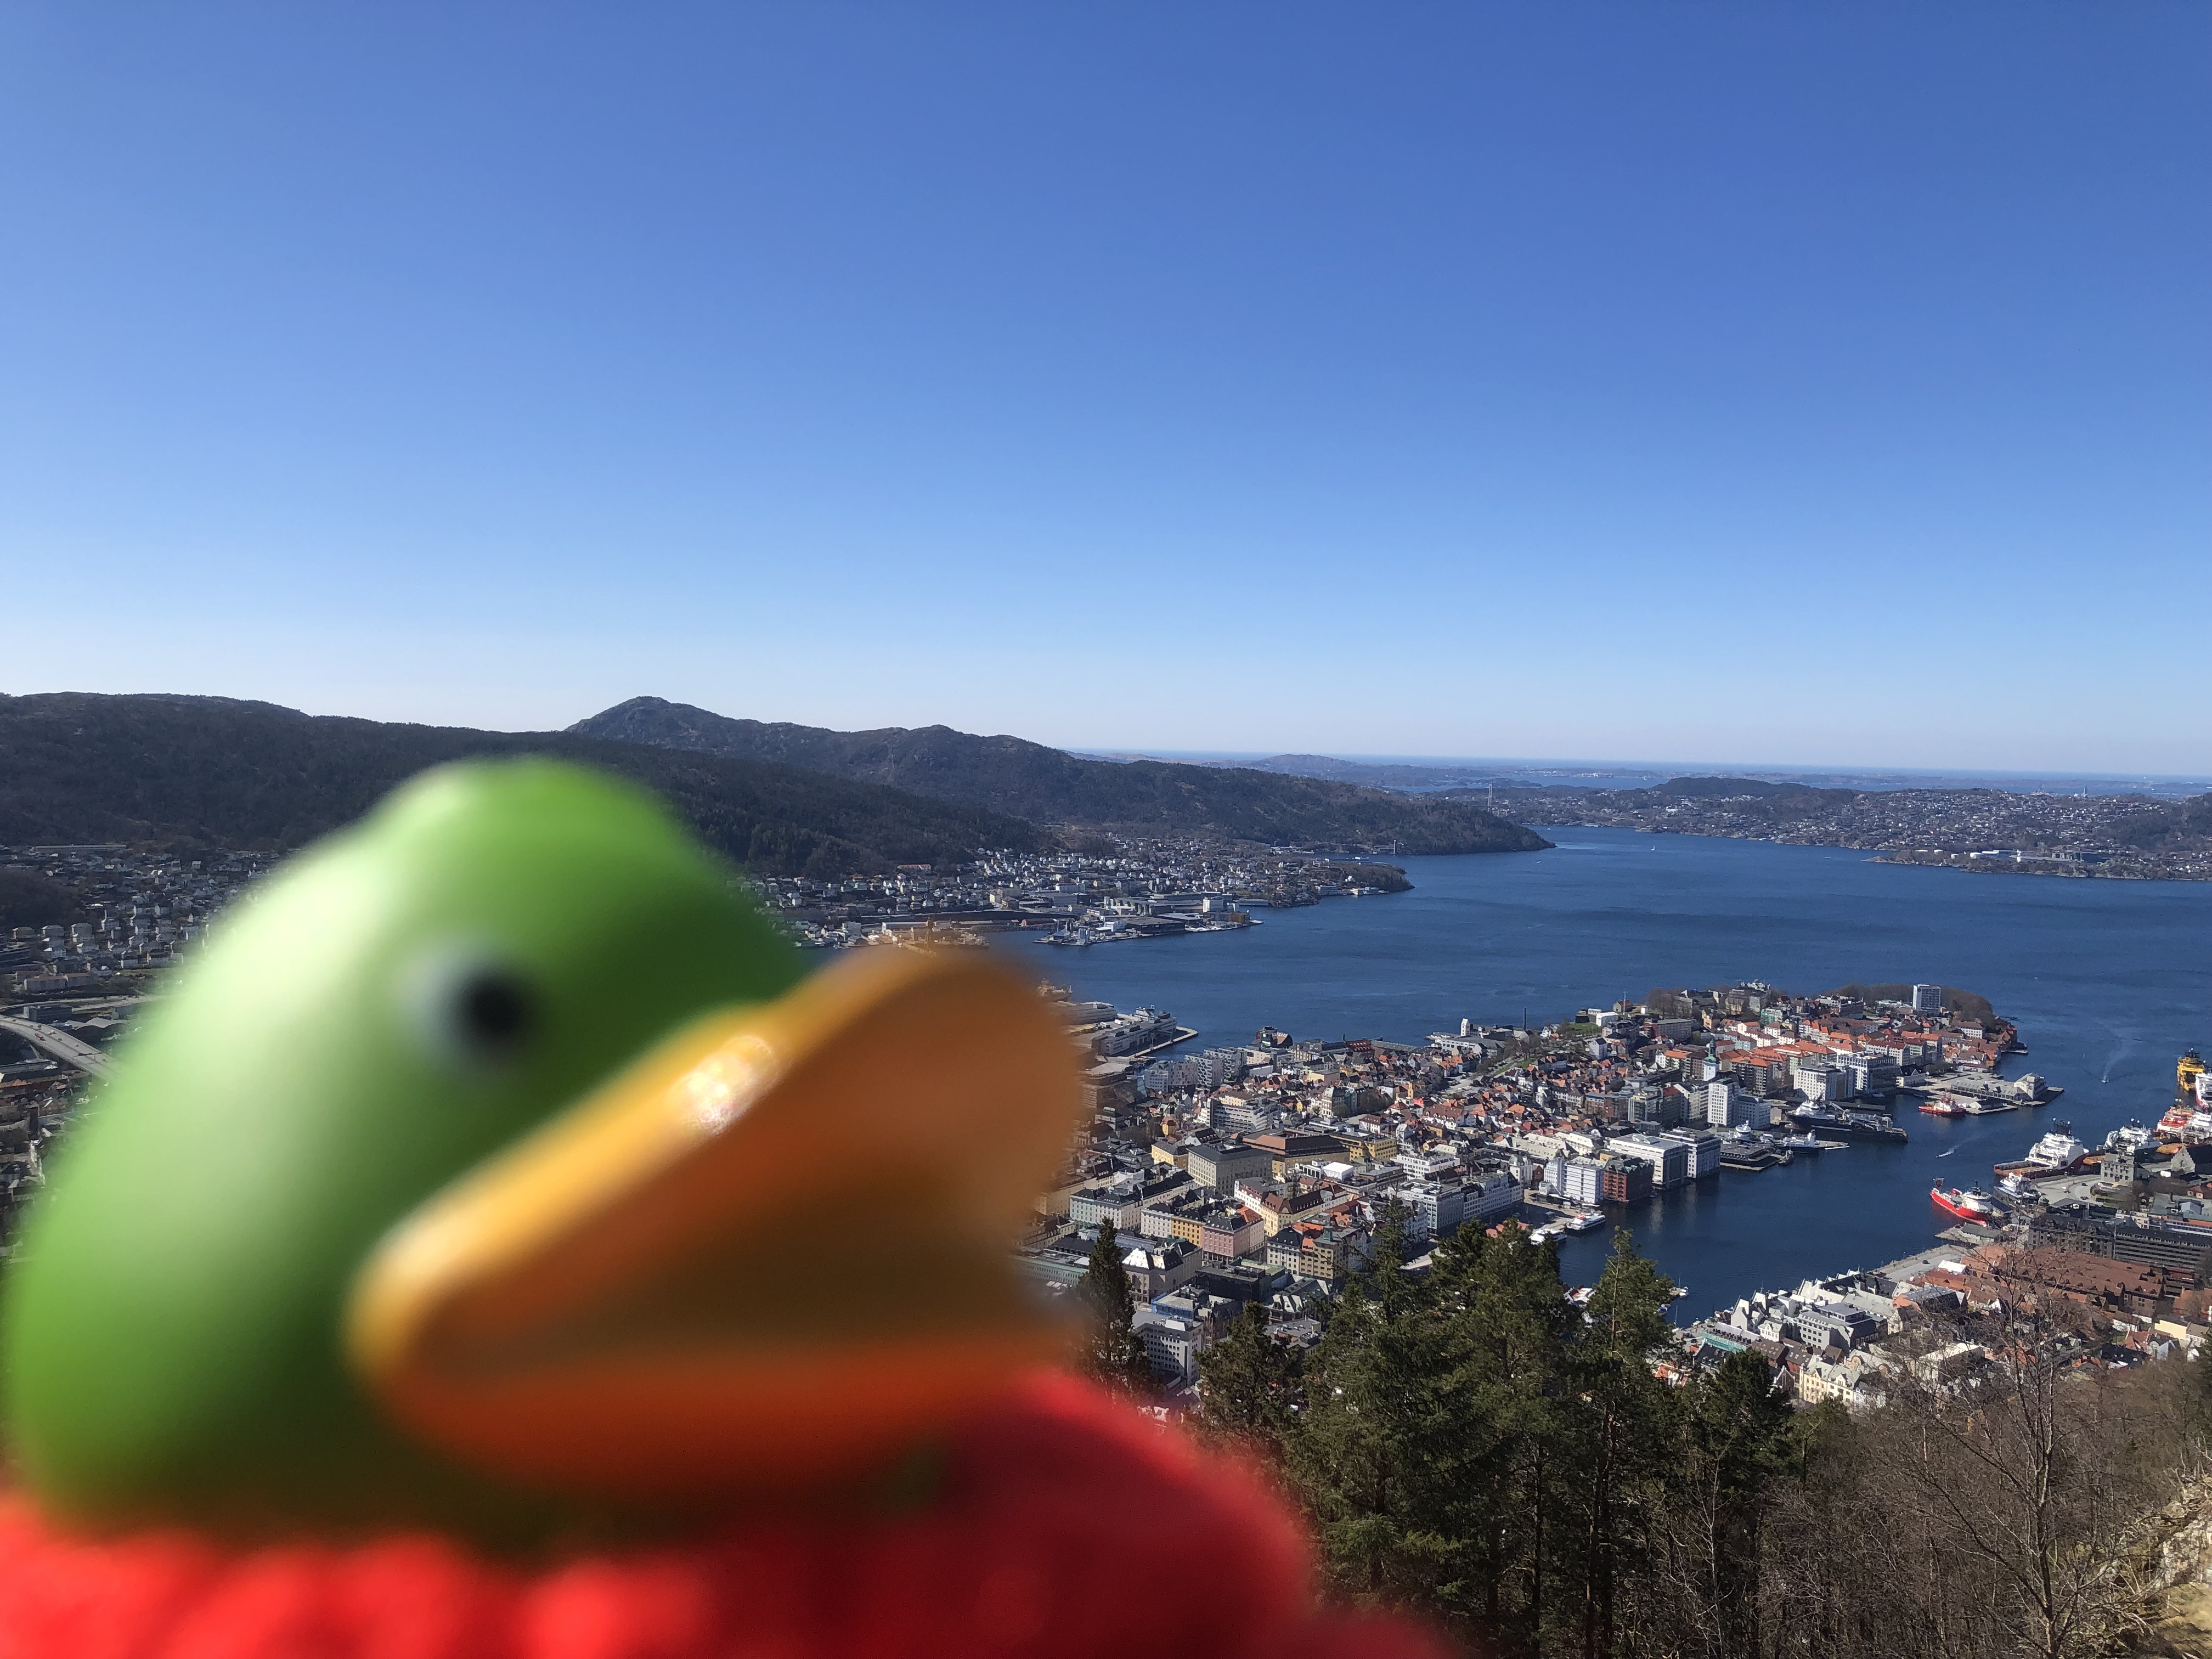
\includegraphics[height = 4.9cm]{images/guillaume10.jpg}
        \caption{Guillaume på Fløyen}
        \label{fig:guillaume10}
    \end{figure}
\end{frame}

\section{Transaksjoner}
\begin{frame}{Hvorfor Transactions?}
    \begin{itemize}[<+->]
        \item Sammenfatte flere kommandoer til en transaksjon
        \item Passe på at alt eller ingenting blir utført
        \item Passe på at flere kommandoer ikke blandes med hverandre
    \end{itemize}
\end{frame}

\begin{frame}{ACID Prinsipper}
    \begin{itemize}[<+->]
        \item Atomicity: Alt eller ingenting blir utført.
        \item Consistency: Databasen går fra en gyldig til en gyldig status.
        \item Isolation: Parallele transaksjoner ser ikke hverandre.
        \item Durability: Resultater av en transaksjon blir ikke overskrevet av den neste transaksjonen.
    \end{itemize}
\end{frame}

\subsection*{Ting som kan gå galt}
\begin{frame}{}
    \begin{block}{Lost Update}
    To transaksjoner jobber på samme tall på samme tidspunkt og den ene overskrever den andres verdien.
    \end{block}
    \pause
    \begin{itemize}[<+->]
        \item Vi får samtidig 1.000 kr fra bestemoren (A) og betaler 100kr til hvem som helst (B)
        \item A leser verdien på kontoen (5000kr)
        \item B leser verdien på kontoen (5000kr)
        \item A legger til 1.000kr og skriver verdien tilbake til databasen (6000kr)
        \item B fjerner 100kr og skriver verdien tilbake til databasen (4900kr)
        \item B har overskrevet resultatet til A
    \end{itemize}
    
\end{frame}

\begin{frame}{}
    \begin{block}{Aborted Update}
    En kommando ikke blir tilbakegjort etter rollback.
    \end{block}
    \pause
    \begin{itemize}[<+->]
        \item A sender 100kr til B
        \item Banken fjerner 100kr fra kontoen til A
        \item Det skjer en feil når man gir 100kr til B
        \item Nå har A tapt 100kr, men B ikke fått 100kr
        \item Databasen må nå rette kontoen til A
    \end{itemize}
\end{frame}

\begin{frame}{}
    \begin{block}{Inconsistent Analysis}
    En kommando baserer seg på både gamle data og nye data samtidig.
    \end{block}
    \pause
    \begin{itemize}[<+->]
        \item Vi skal legge til en film og en screening i databasen
        \item I tillegg skal vi få en joined tabell med alle filmer og screenings til sammen
        \item Hvis man legger til film, kjører JOIN kommandoen og etterpå legger til screening, har vi \textit{inconsistent analysis}
        \item Kommandoen baserer informasjoner på gamle verdier (screening tabell) og nye verdier (film database) samtidig
        \item Enten gjør alle INSERT på begynnelsen eller på slutten
    \end{itemize}
\end{frame}

\subsection*{SQL Transaksjoner}
\begin{frame}[fragile]{Transaksjoner i SQL}
\begin{minted}{sql}
START TRANSACTION;      -- her starter transaksjonen
UPDATE bankaccount      -- ta 20kr fra en bankkonto 
SET money = money - 20  -- dette er ikke korrekt syntaks
WHERE customer = 42;
UPDATE bankaccount      -- gi de 20kr til en annen bankkonto
SET money = money + 20
WHERE customer = 20;
COMMIT;                 -- commit hvis alt gikk fint, ellers rollback
-- ROLLBACK
\end{minted}
\end{frame}

\subsection*{Begrep}
\begin{frame}
\begin{itemize}[<+->]
    \item Serialisability: To transaksjoner er serialisable dersom det finnes en rekkefølge de kan utføres uten at de ignorerer ACID-prinsippene
    \item Write lock: Variabel kan ikke endres, men verdien kan leses 
    \item Read lock: Variabel kan verken leses eller endres
    \item Two phase locking: Blokker alle variabler samtidig, frigir dem samtidig
\end{itemize}
\end{frame}

\subsection*{Waiting graph}
\begin{frame}{Finn rekkefølge for transaksjoner}
\begin{itemize}[<+->]
    \item Lag rettet graf med transaksjoner som noder
    \item A venter til B: $A \rightarrow B$ (retningen antiintuitiv)
    \item Finn en rekkefølge å gå gjennom nodene
    \item Hvis graf har sykler finnes ikke en sånn rekkefølge
    \item Fjern de eldste transaksjonene inntil ingen sykler er igjen
\end{itemize}
\end{frame}

\begin{frame}{Eksempel}
\begin{columns}
    \begin{column}{0.48\textwidth}
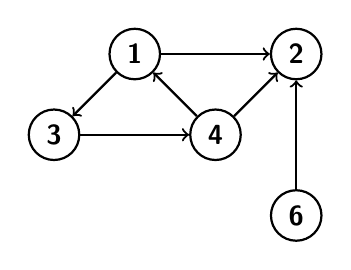
\begin{tikzpicture}[
    node distance=1.45cm, thick,
    main node/.style={circle, draw, font=\sffamily\bfseries}
]
    \node<-4>[main node] (1)                    {1};
    \node[main node,onslide=<8>{fill=black!60!green}] (3) [below left  of=1] {3};
    \node[main node,onslide=<7->{fill=black!60!green}] (4) [below right of=1] {4};
    \node[main node,onslide=<3->{fill=black!60!green}] (2) [above right of=4] {2};
    \node[main node,onslide=<4->{fill=black!60!green}] (6) [below right of=4] {6}; % <-4> forces an additional overlay in which node 2 disappears

    \path<1>[->] (1) edge (2)
        (4) edge (2)
        (6) edge (2);
    \path<-4>[->] (1) edge (3)
        (4) edge (1);
    \path<-5>[->] (3) edge (4);
\end{tikzpicture}
 \end{column}
    \begin{column}{0.48\textwidth}
\begin{itemize}
    \item<1-> Graf med fem noder 
    \item<2-> Transaksjon 2 venter på ingenting
    \item<3-> Marker transaksjon 2 som utført
    \item<4-> Marker transaksjon 6 som utført
    \item<5-> Funnet syklus, fjern eldeste transaksjon 1
    \item<6-> Transaksjon 4 venter på ingenting
    \item<7-> Marker transaksjon 4 som utført
    \item<8-> Marker transaksjon 3 som utført
\end{itemize}
 \end{column}
\end{columns}
\end{frame}

\subsection*{Spørretid}
\begin{frame}{Spørsmål?}
    \begin{figure}
        \centering
        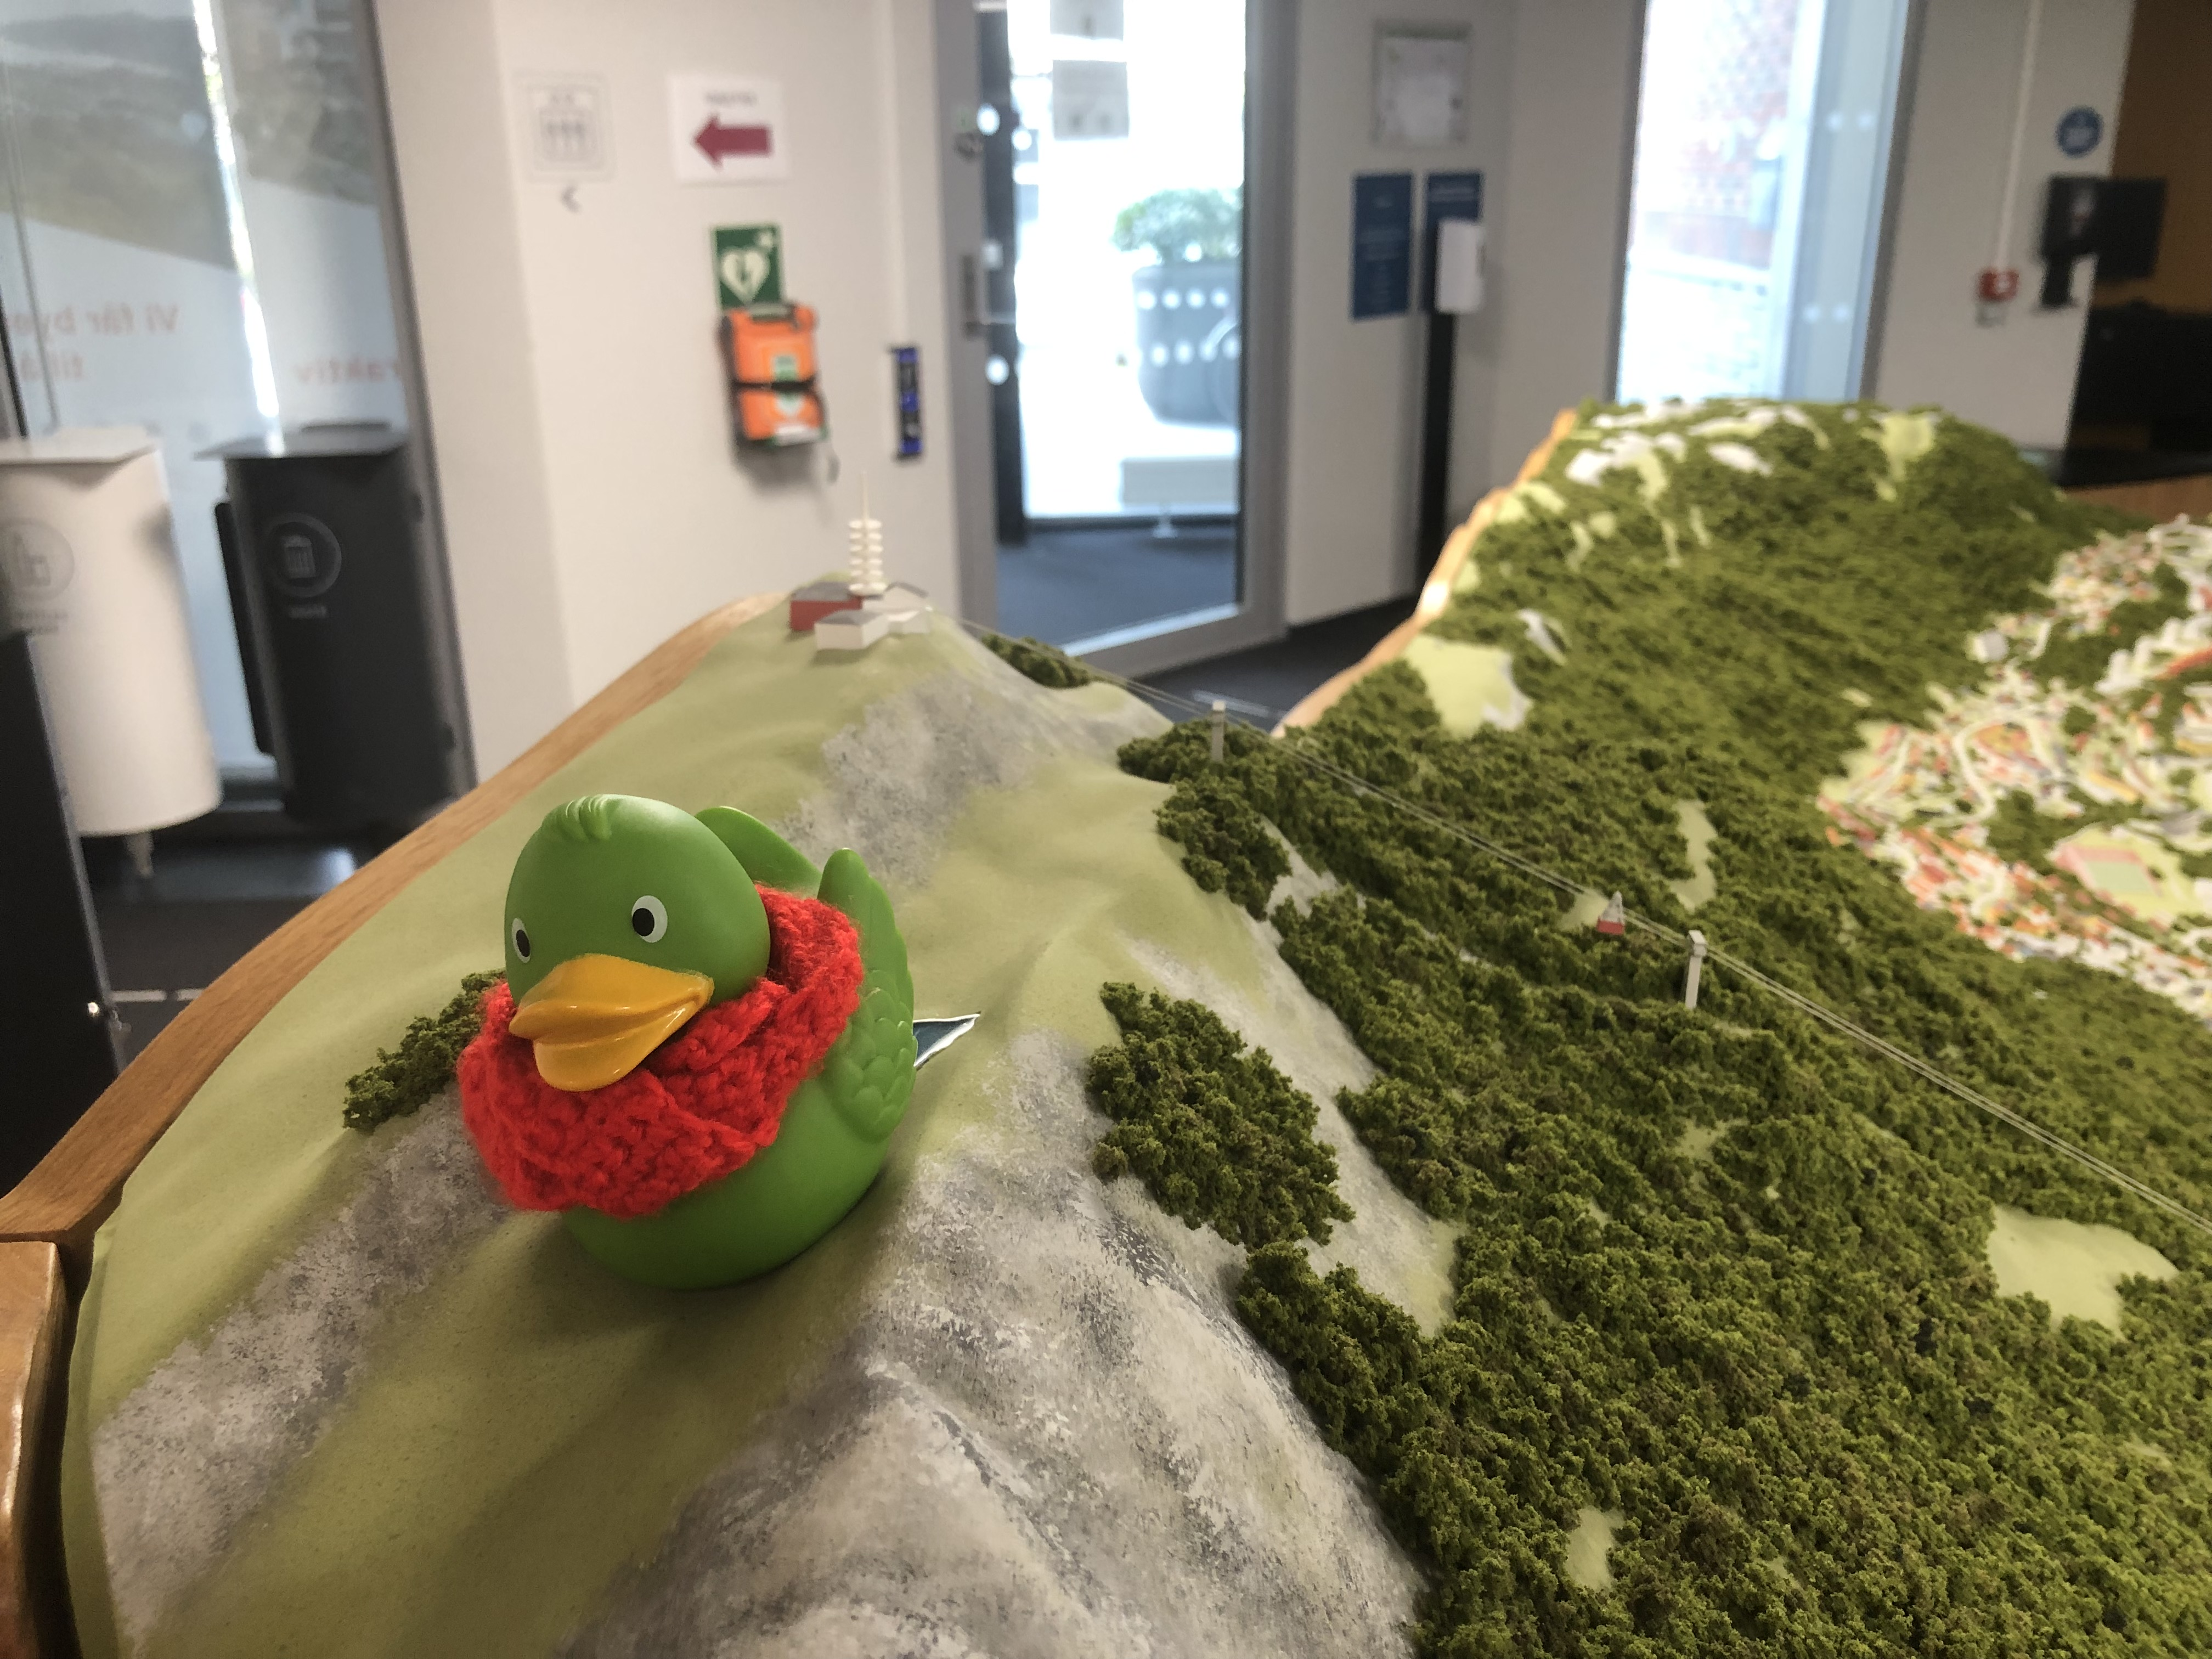
\includegraphics[height = 4.9cm]{images/guillaume11.jpg}
        \caption{Guillaume på Ulriken}
        \label{fig:guillaume11}
    \end{figure}
\end{frame}

\section{Alt mulig}
\begin{frame}{Andre teamer}
\begin{itemize}[<+->]
    \item Databaseadministrasjon
    \item Webapplikasjoner (php, tragisk)
    \item NoSQL, XML, JSON
    \item Noen småteamer og informasjoner fra temaene i kræsjkurset
    \item Guest Lectures
\end{itemize}
\end{frame}

\subsection*{Spørretid}
\begin{frame}{Spørsmål?}
    \begin{figure}
        \centering
        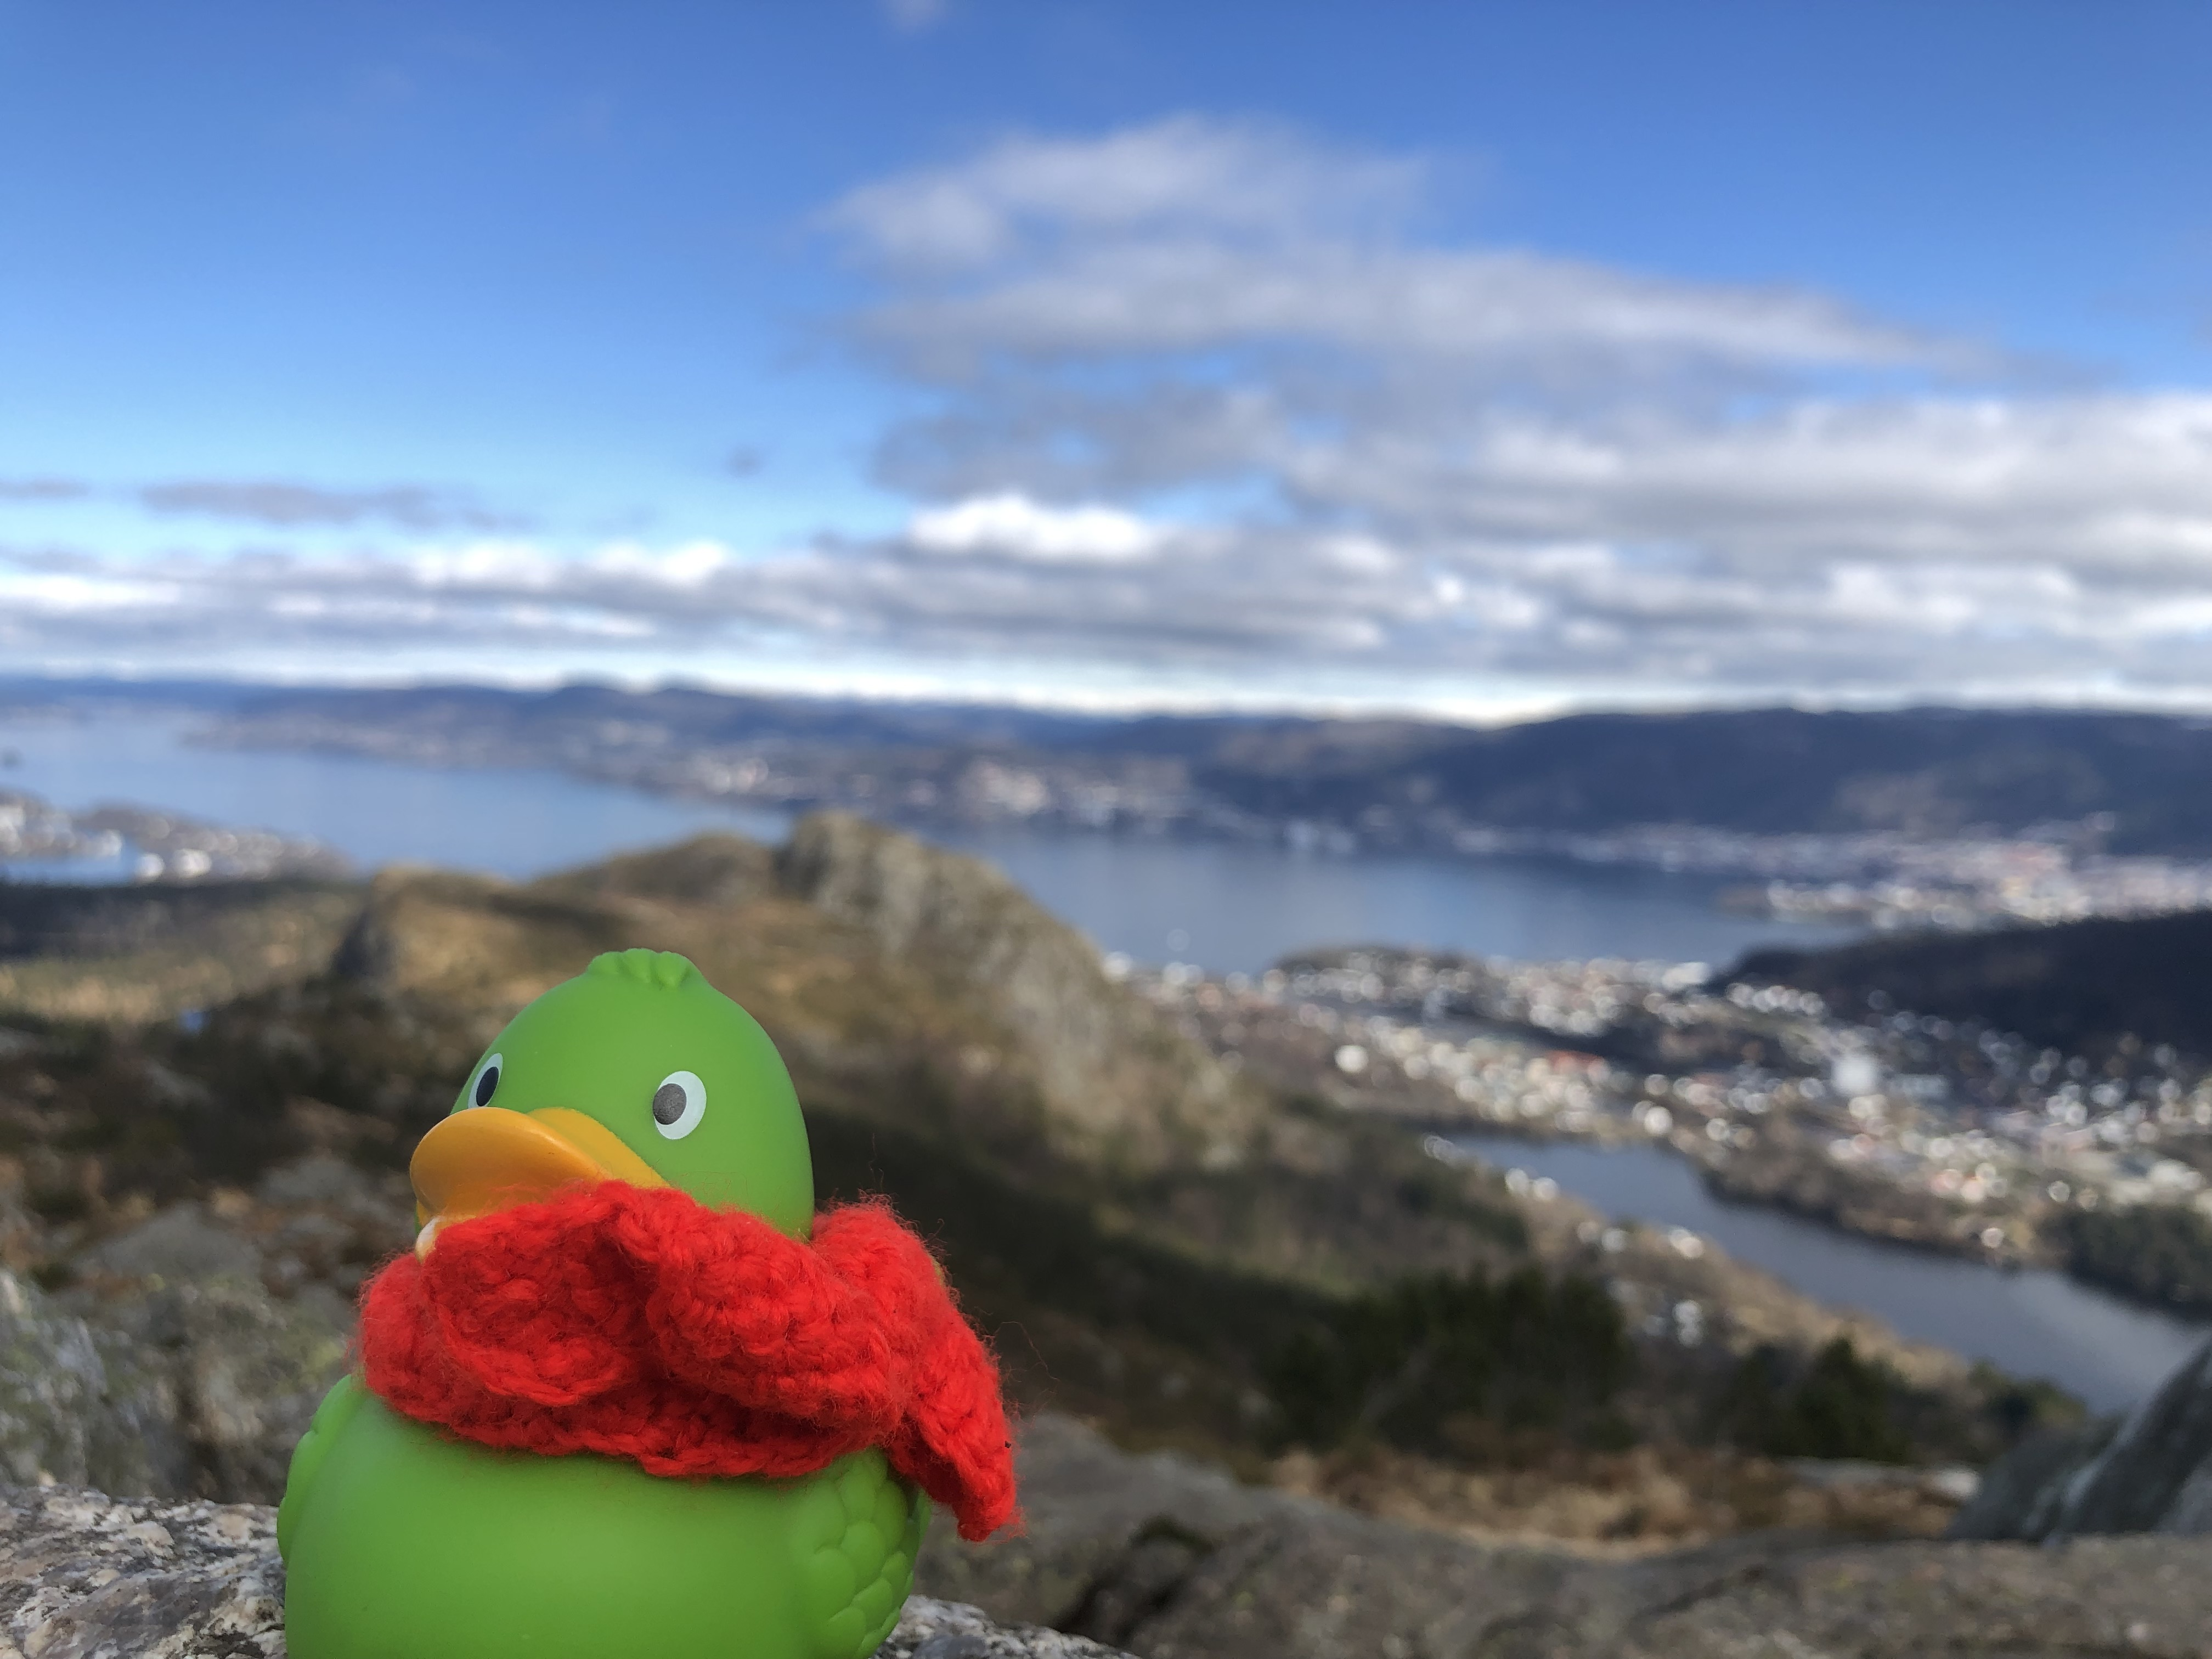
\includegraphics[height = 4.9cm]{images/guillaume8.jpg}
        \caption{Guillaume på Lyderhorn}
        \label{fig:guillaume8}
    \end{figure}
\end{frame}

\subsection*{Tilbakemeldingsskjema}
\begin{frame}{Tilbakemeldinger ønsket!}
    \begin{figure}
        \centering
        
\includegraphics[height = 4.9cm]{images/qrtilbakemelding.png}
        \caption{https://tinyurl.com/inf115tmv23}
        \label{fig:qrcodetilbakemelding}
    \end{figure}
\end{frame}

%\section*{Slutt}
\begin{frame}
\begin{center}
\begin{Large}
\textbf{Lykke til på eksamen!\\[5mm]
Takk for meg}
\end{Large}
\end{center}  
\end{frame}

\end{document}
